\section{Trigger \label{sec:trigger}}
As discussed in Sec.~\ref{sec:computing}, in order for an event to be triggered for readout it must pass one of a collection of algorithms.
The data used in this chapter is required to have been collected by triggers looking for a high momentum track to be found
and/or missing transverse energy, MET, as calculated by the particle flow algorithm~\cite{Chatrchyan:2011tn}. 

The particle flow algorithm attempts
to reconstruct all particles in an event, then calculates MET as the magnitude of the negative vector sum of the transverse momenta of the particles. 
The MET calculated by the particle flow algorithm is referred to as PFMET.
As the proton-proton collision occurs
at rest in the transverse plane, PFMET is meant to represent the magnitude of the vector sum of all particles not found by the particle flow algorithm.
In particular, PFMET is intended to measure the transverse momentum of neutral particles in the event which leave no signals in the detector.
These neutral particles could be neutrinos from the SM or new neutral particles created in a BSM theory such as supersymmetry.
In practice, PFMET can also be created by the limited detector response in finding all tracks in an event and determining their momentum.

For HSCP, additional contributions to PFMET often arise because of details of the particle flow algorithm.
The algorithm assumes SM particles and rejects reconstructed tracks that do not conform to the properties expected
of a SM particle. Two types of possible HSCP tracks are rejected by the algorithm. 

The first type is tracks reconstructed only in the muon system. The only charged SM particles that
are expected to reach the muon system are muons. As muons should have a matching track in the inner tracker, particle flow rejects tracks found only in the
muon system. HSCP produced neutral then acquiring charge by interacting with the calorimeter
would only have a track in the muon system and as such would not be included in the PFMET calculation. 

The second type is tracks produced charged but becoming neutral as they propagate through CMS.
The particle flow algorithm rejects tracks reconstructed only in the inner tracker that have a track $p_T$ much larger
than the associated energy deposited in the calorimeter as this indicates the track has been misreconstructed.
As an HSCP only deposits approximately 10~GeV of energy in the calorimeter and normally has $>$ 100~GeV/$c$ of momentum, HSCP neutral in the muon system will likely be rejected. 

These two effects lead to PFMET in HSCP events to be roughly equal to the vector sum of any $R$--hadrons neutral in
either the muon system or the inner tracker, less however much energy they deposit in the calorimeter. This effect is illustrated in Figures~\ref{fig:SystPtTrigger} 
and~\ref{fig:SystPtTriggerN} which compare the di-HSCP system with the measurement of PFMET
in gluino pair events with at least 150~GeV/$c$ of PFMET. For all instances of PFMET the value is the one determined by the trigger.

\begin{figure}
  \begin{center}
      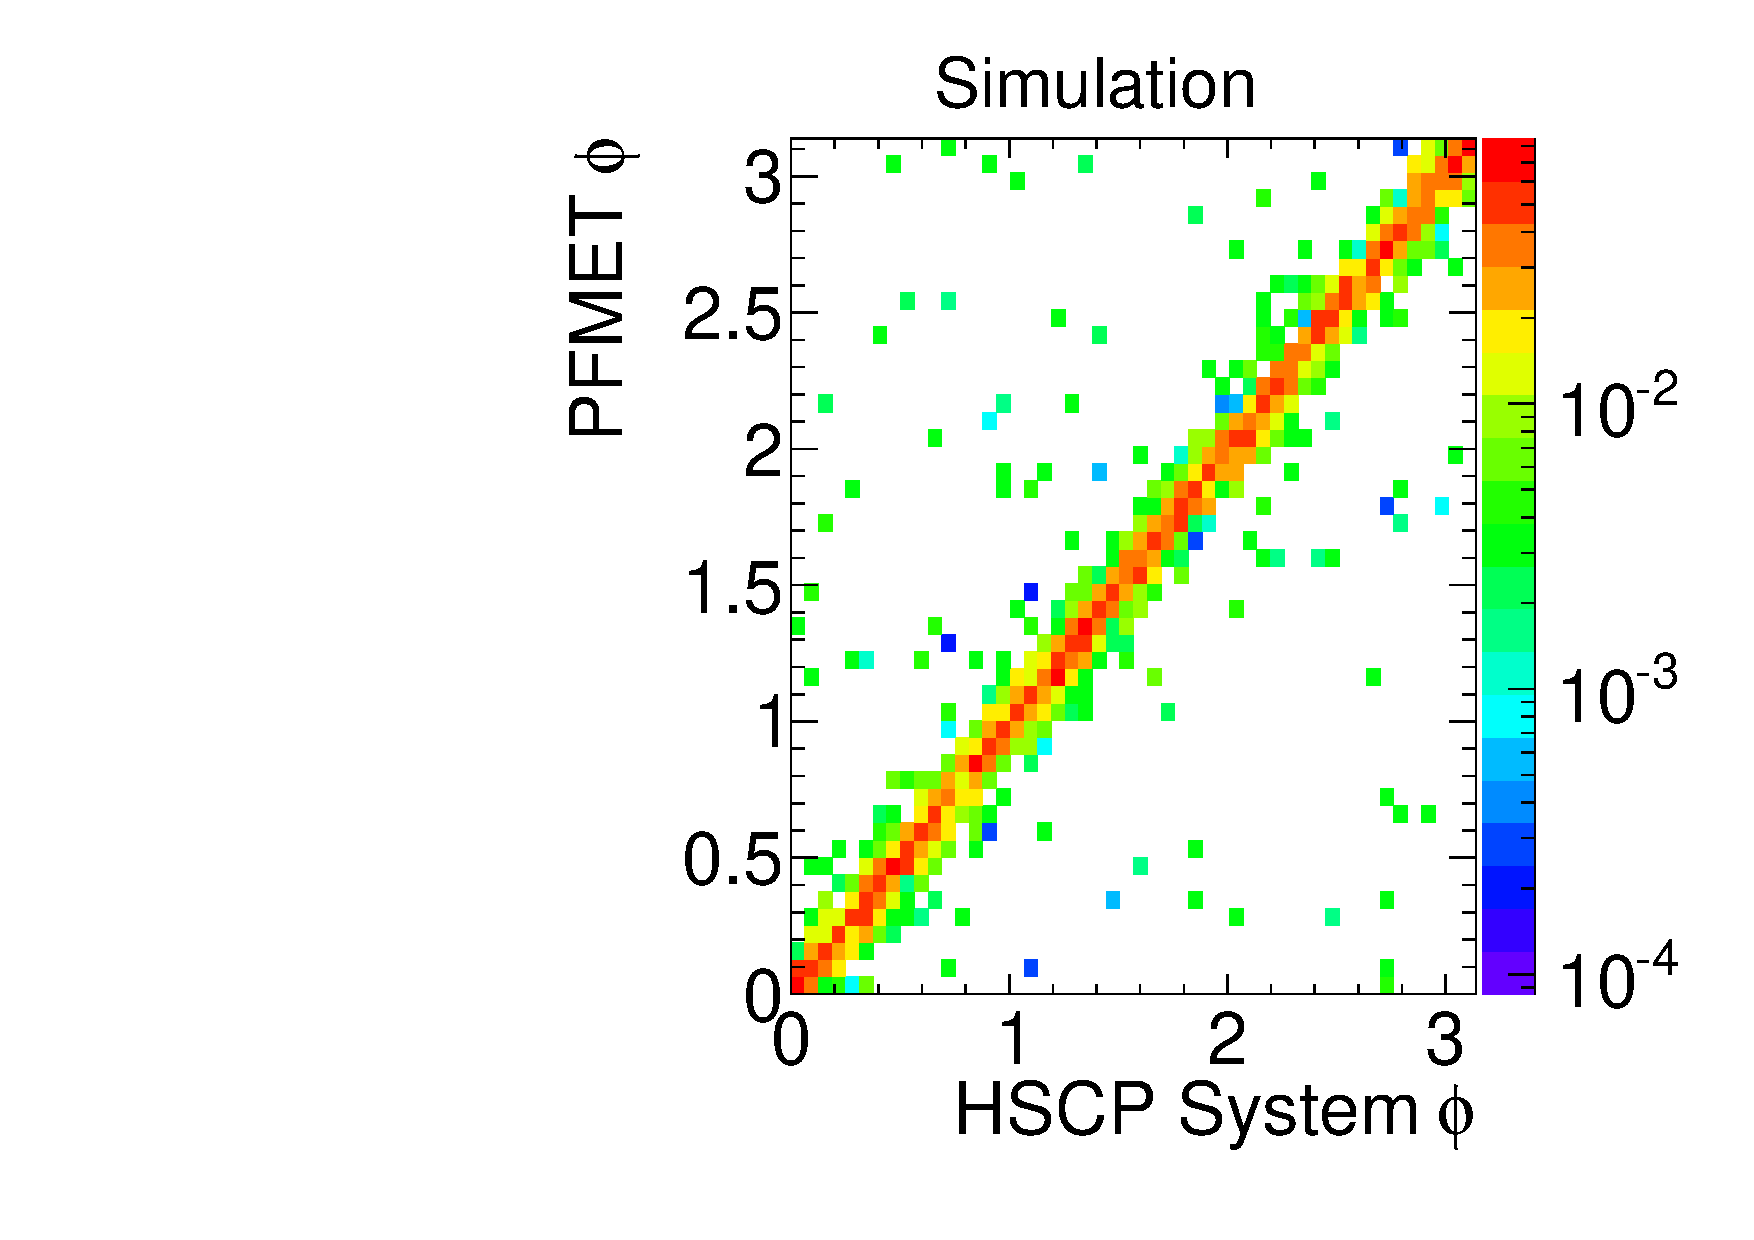
\includegraphics[clip=false, trim=0.0cm 0cm 0.0cm 0cm, width=0.49\textwidth]{figures/search/Gluino_8TeV_M1200_f100SystPhiMET}
      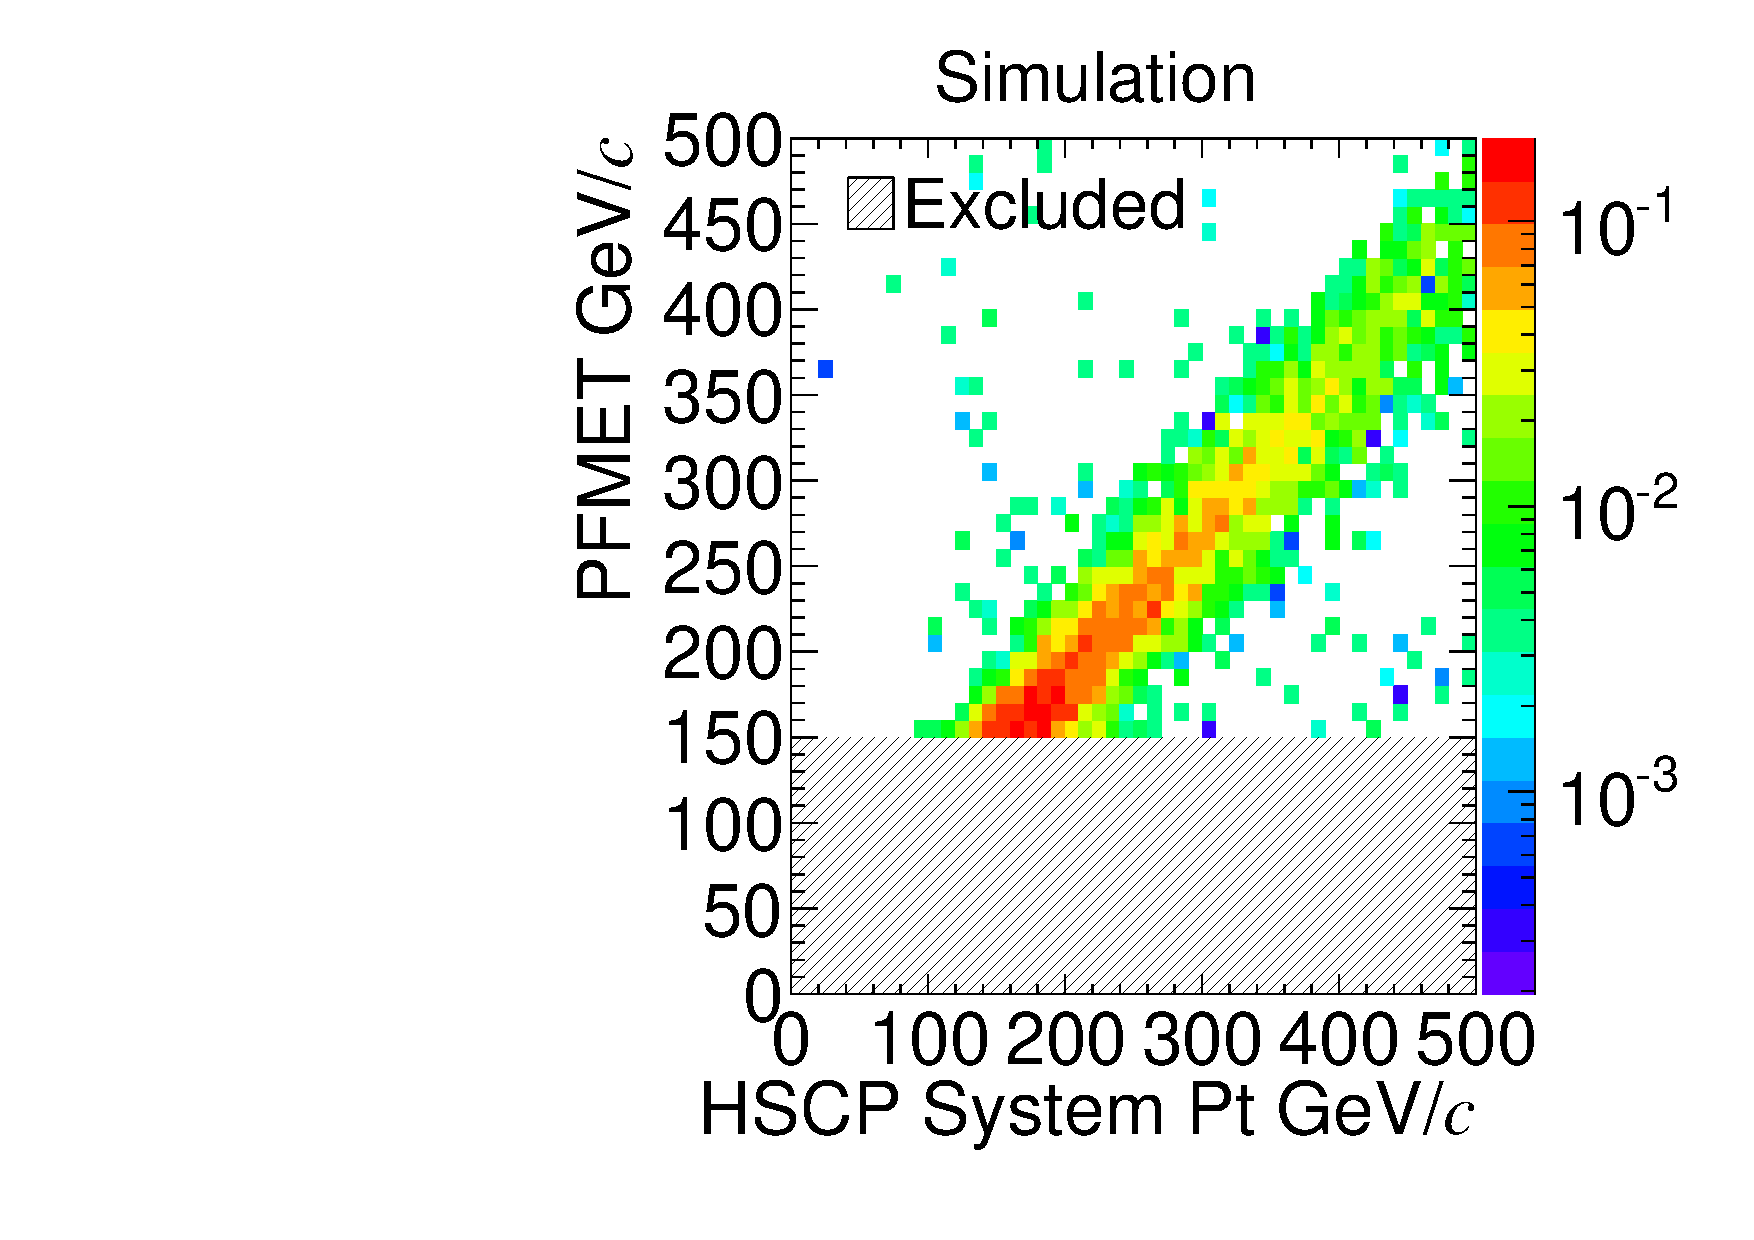
\includegraphics[clip=false, trim=0.0cm 0cm 0.0cm 0cm, width=0.49\textwidth]{figures/search/Gluino_8TeV_M1200_f100SystPtMET} \\
      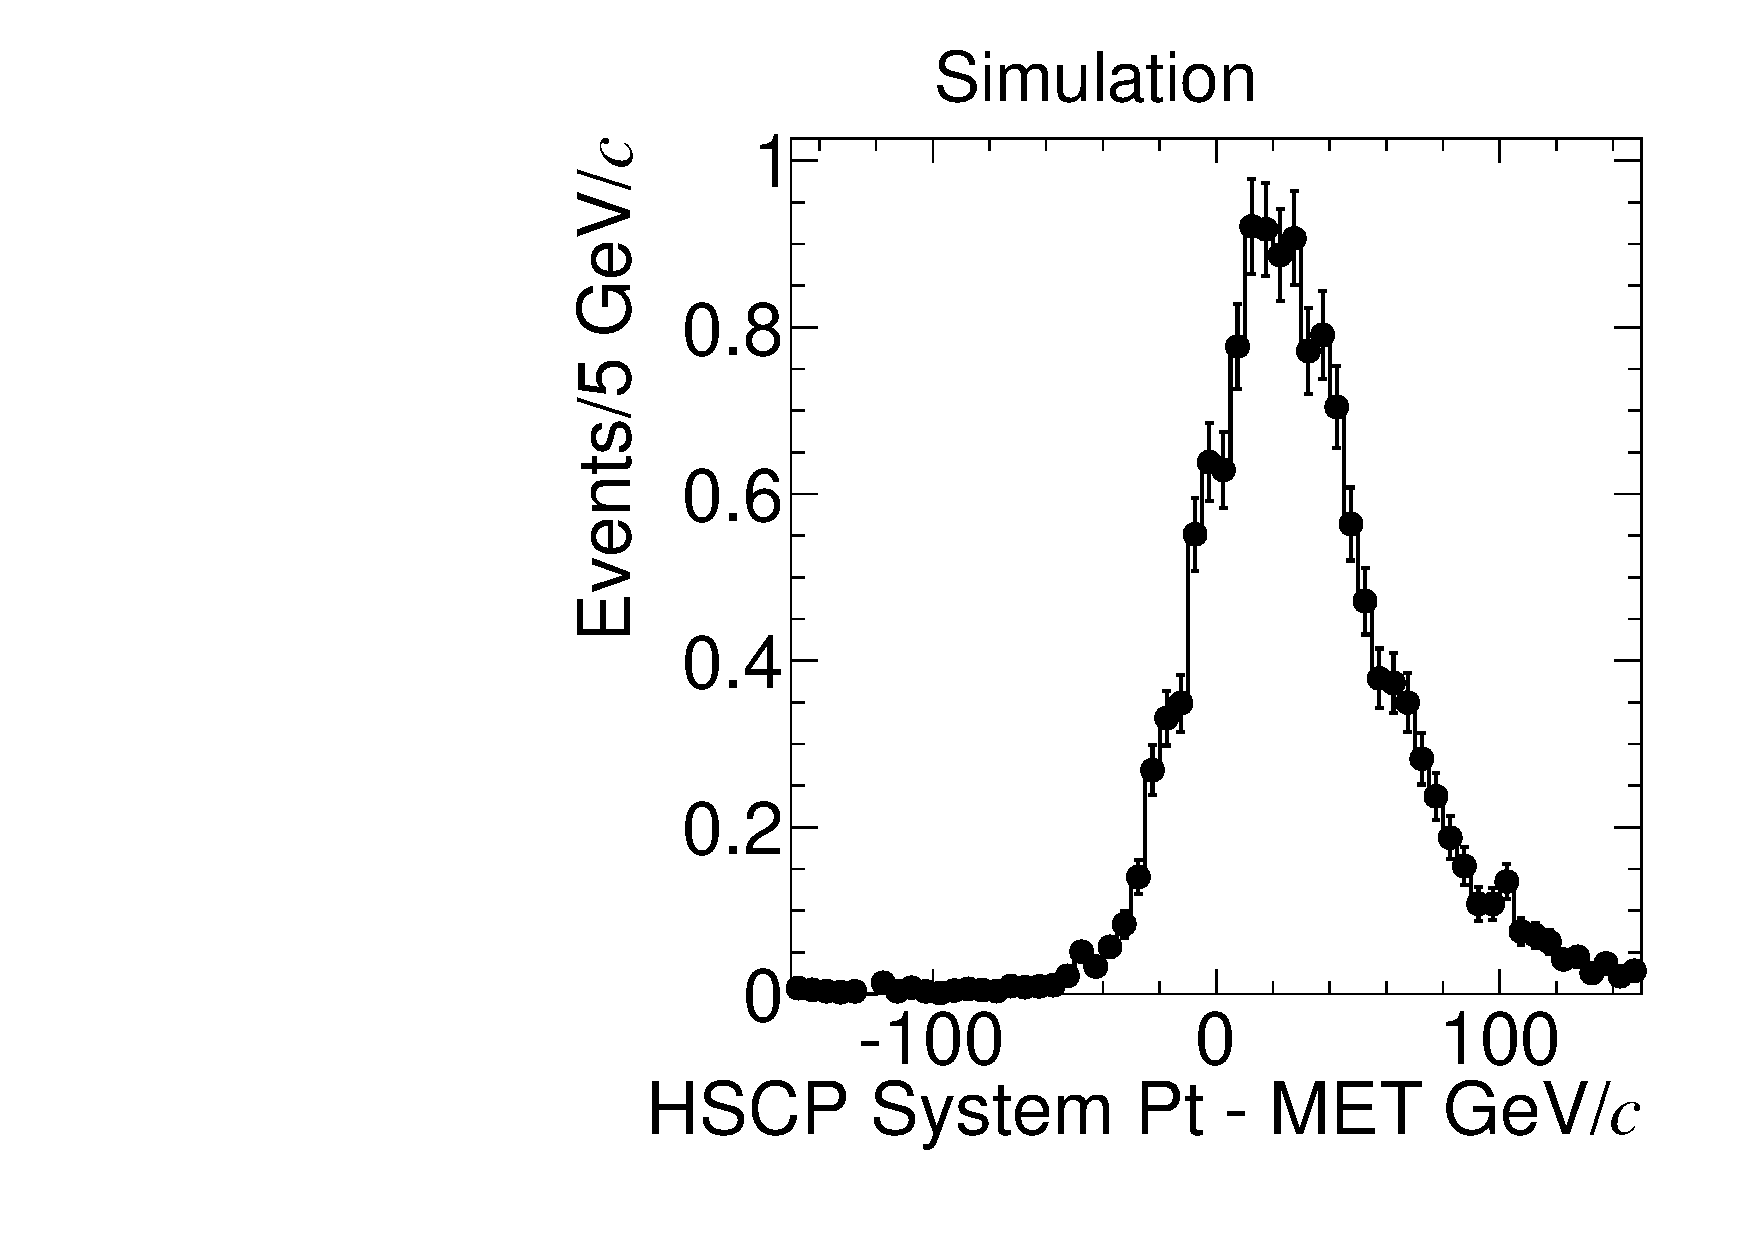
\includegraphics[clip=false, trim=0.0cm 0cm 0.0cm 0cm, width=0.49\textwidth]{figures/search/Gluino_8TeV_M1200_f100SystPtDiffMET}
      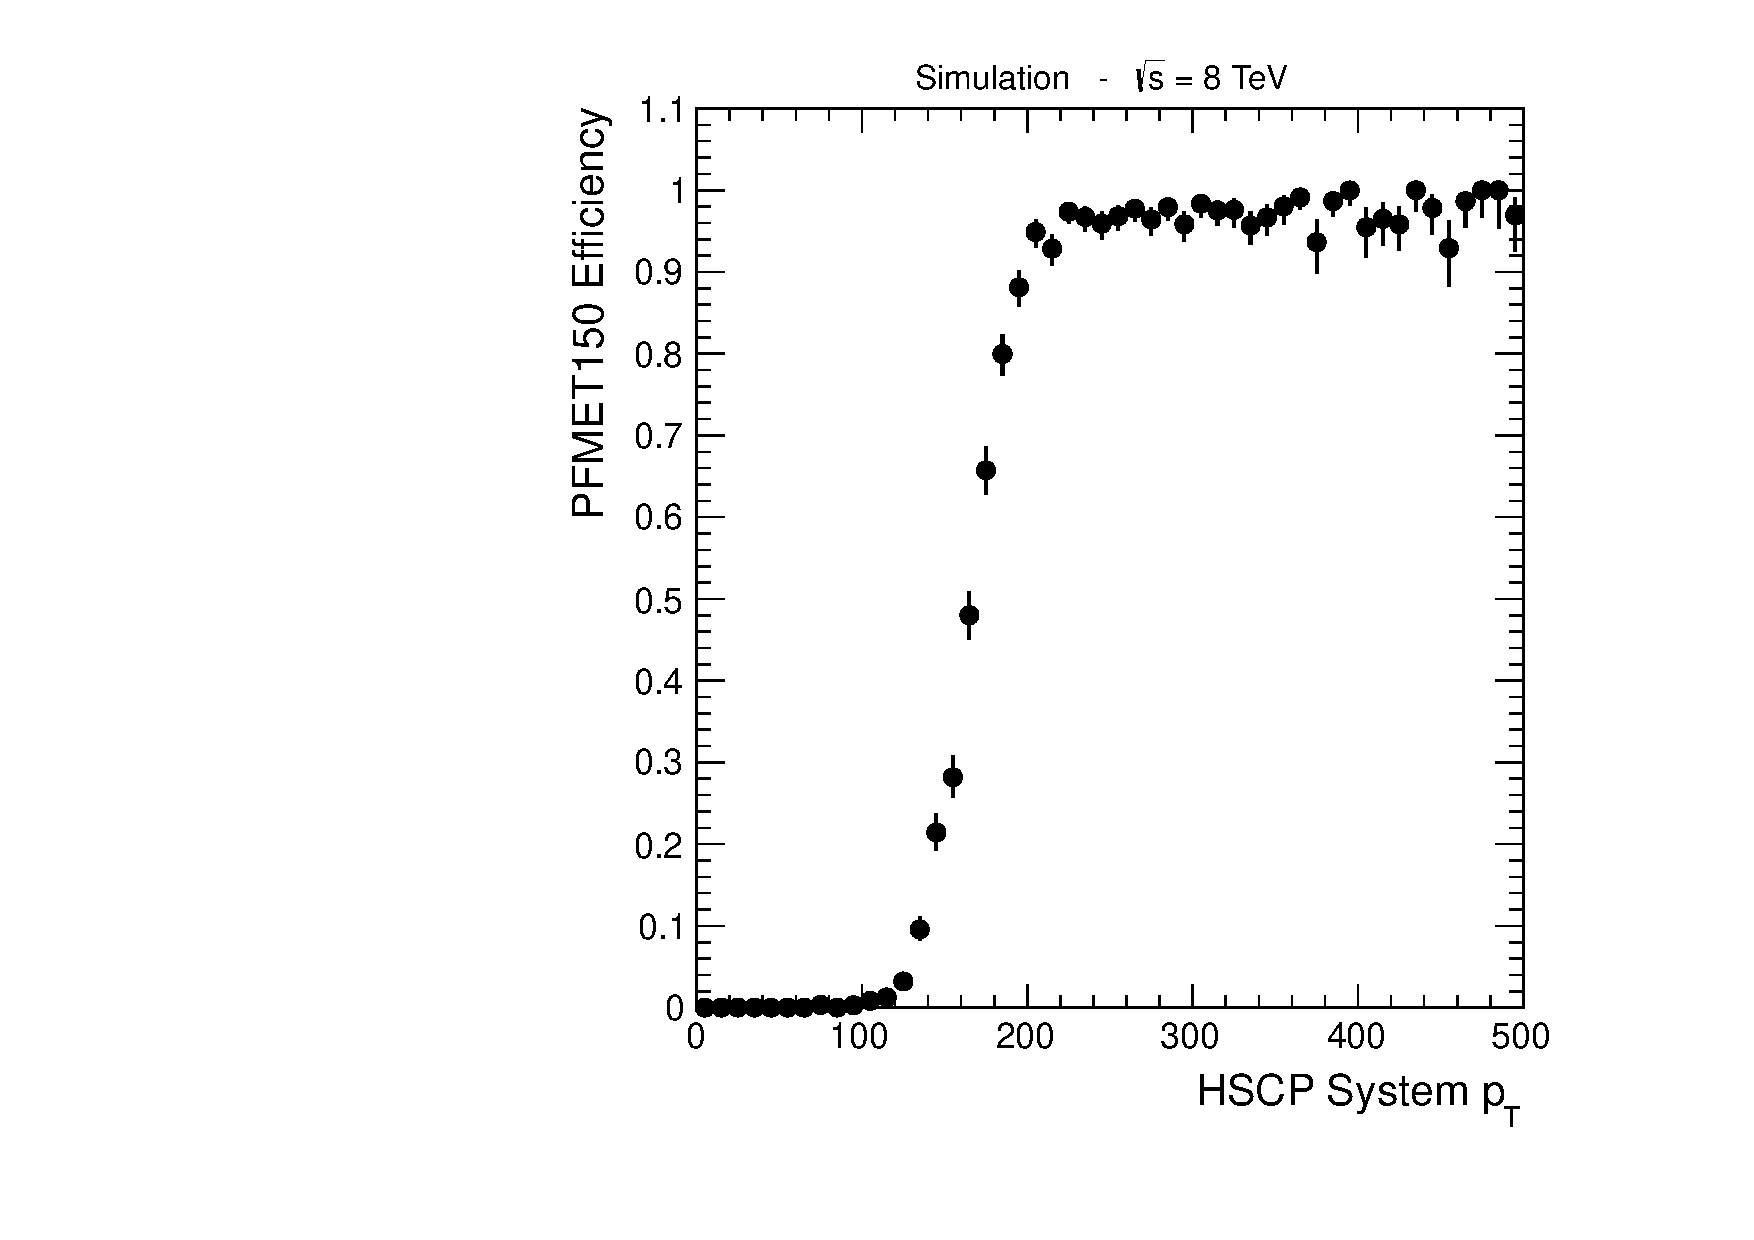
\includegraphics[clip=false, trim=0.0cm 0cm 0.0cm 0cm, width=0.49\textwidth]{figures/search/Gluino_8TeV_M1200_f100SystPtEff}
      \caption[Comparison of di-HSCP system $\phi$ and \pt\ with PFMET for a 1200~GeV/$c^2$ 
gluino $f=1.0$ sample in events with at least 150~GeV/$c$ of PFMET.]
              {Comparison of di-HSCP system with PFMET for a 1200~GeV/$c^2$ gluino $f=1.0$ sample. For all instancesof PFMET the value is the one determined by thetrigger.
		All figures but the bottom right one only consider events with at least 150~GeV/$c$ of PFMET. 
         Top Left: PFMET $\phi$ versus di-HSCP system $\phi.$ Top Right: PFMET value versus di-HSCP system $p_T$. 
         Bottom Left: Difference between di-HSCP system $p_T$ and PFMET value.
         Bottom Right: Probability to have PFMET greater than 150~GeV/$c$ versus di-HSCP system $p_T$. A horizontal dashed line is drawn at one.
        }
      \label{fig:SystPtTrigger}
  \end{center}
\end{figure}

\begin{figure}
  \begin{center}
      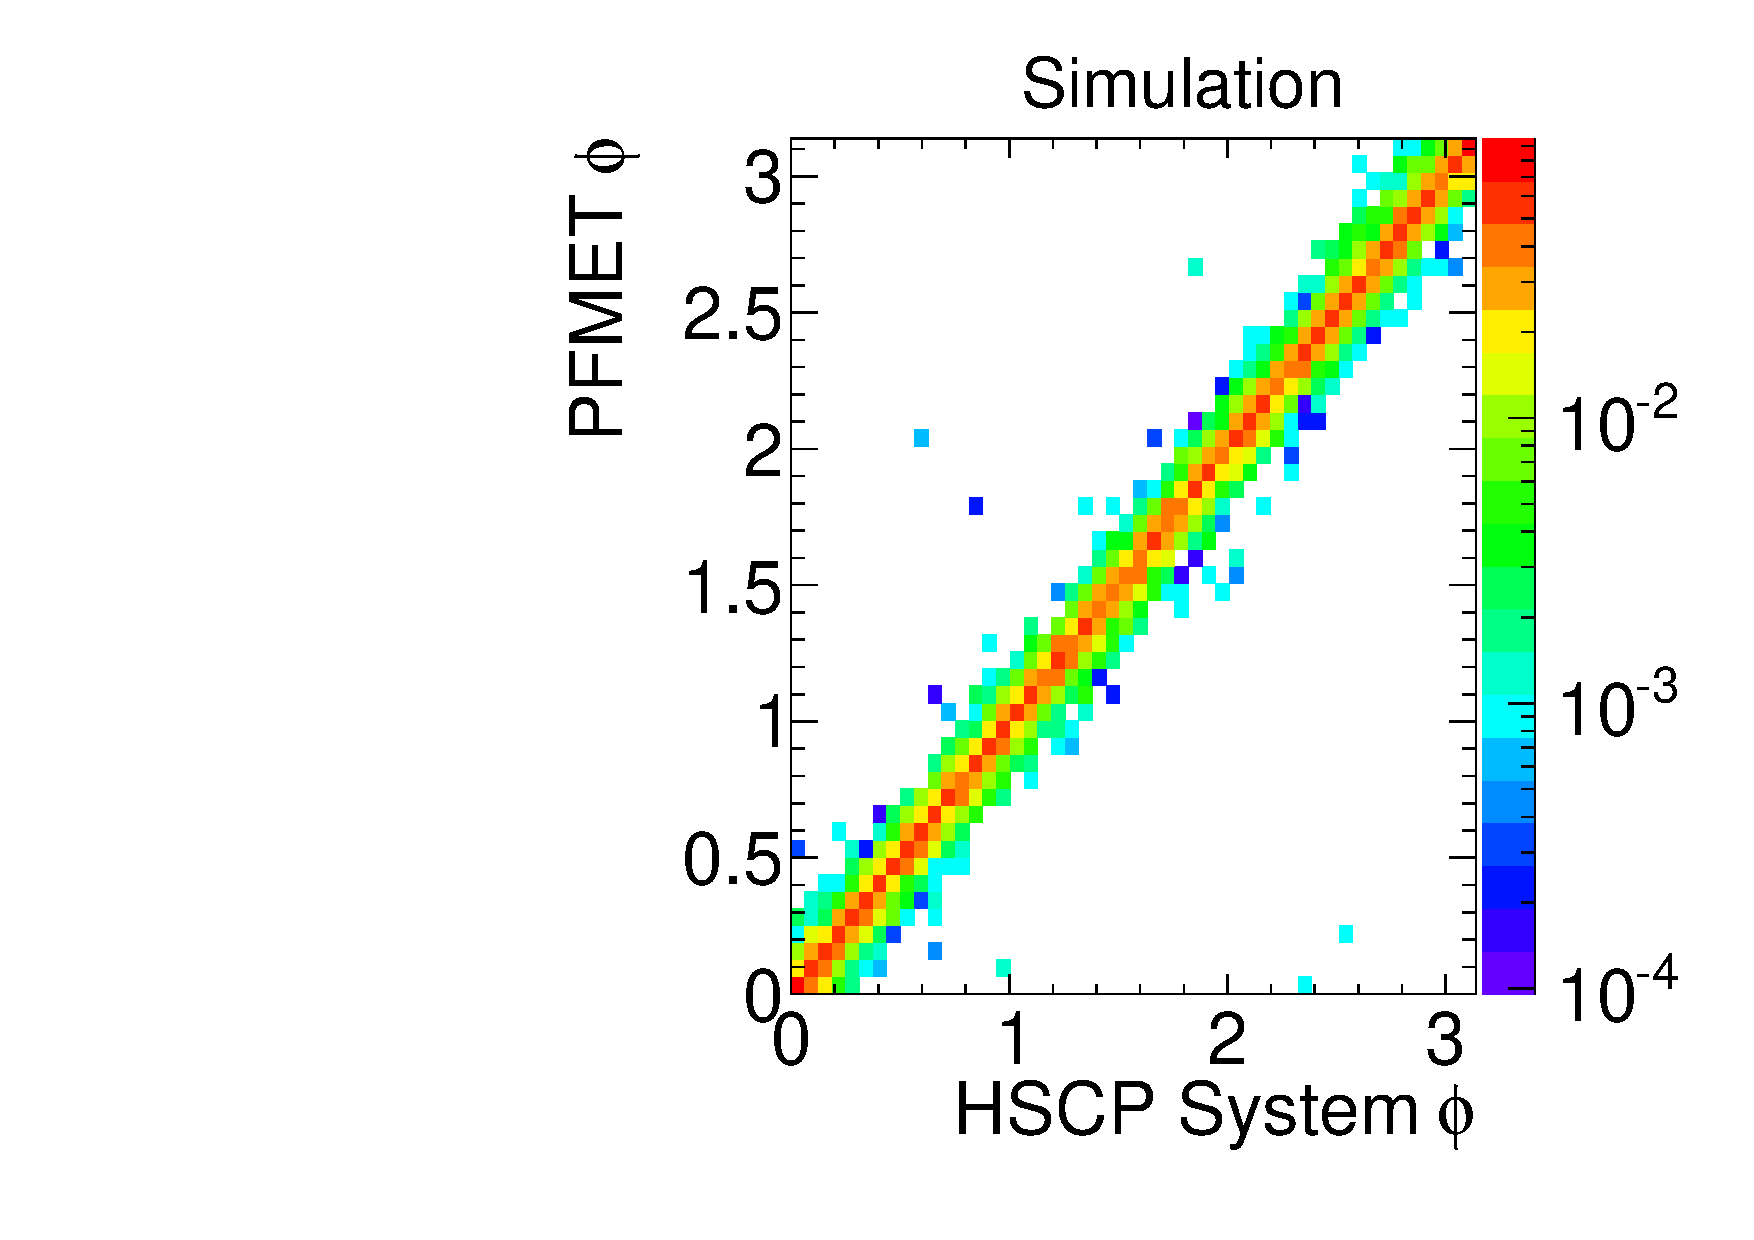
\includegraphics[clip=false, trim=0.0cm 0cm 0.0cm 0cm, width=0.49\textwidth]{figures/search/Gluino_8TeV_M1200N_f10SystPhiMET}
      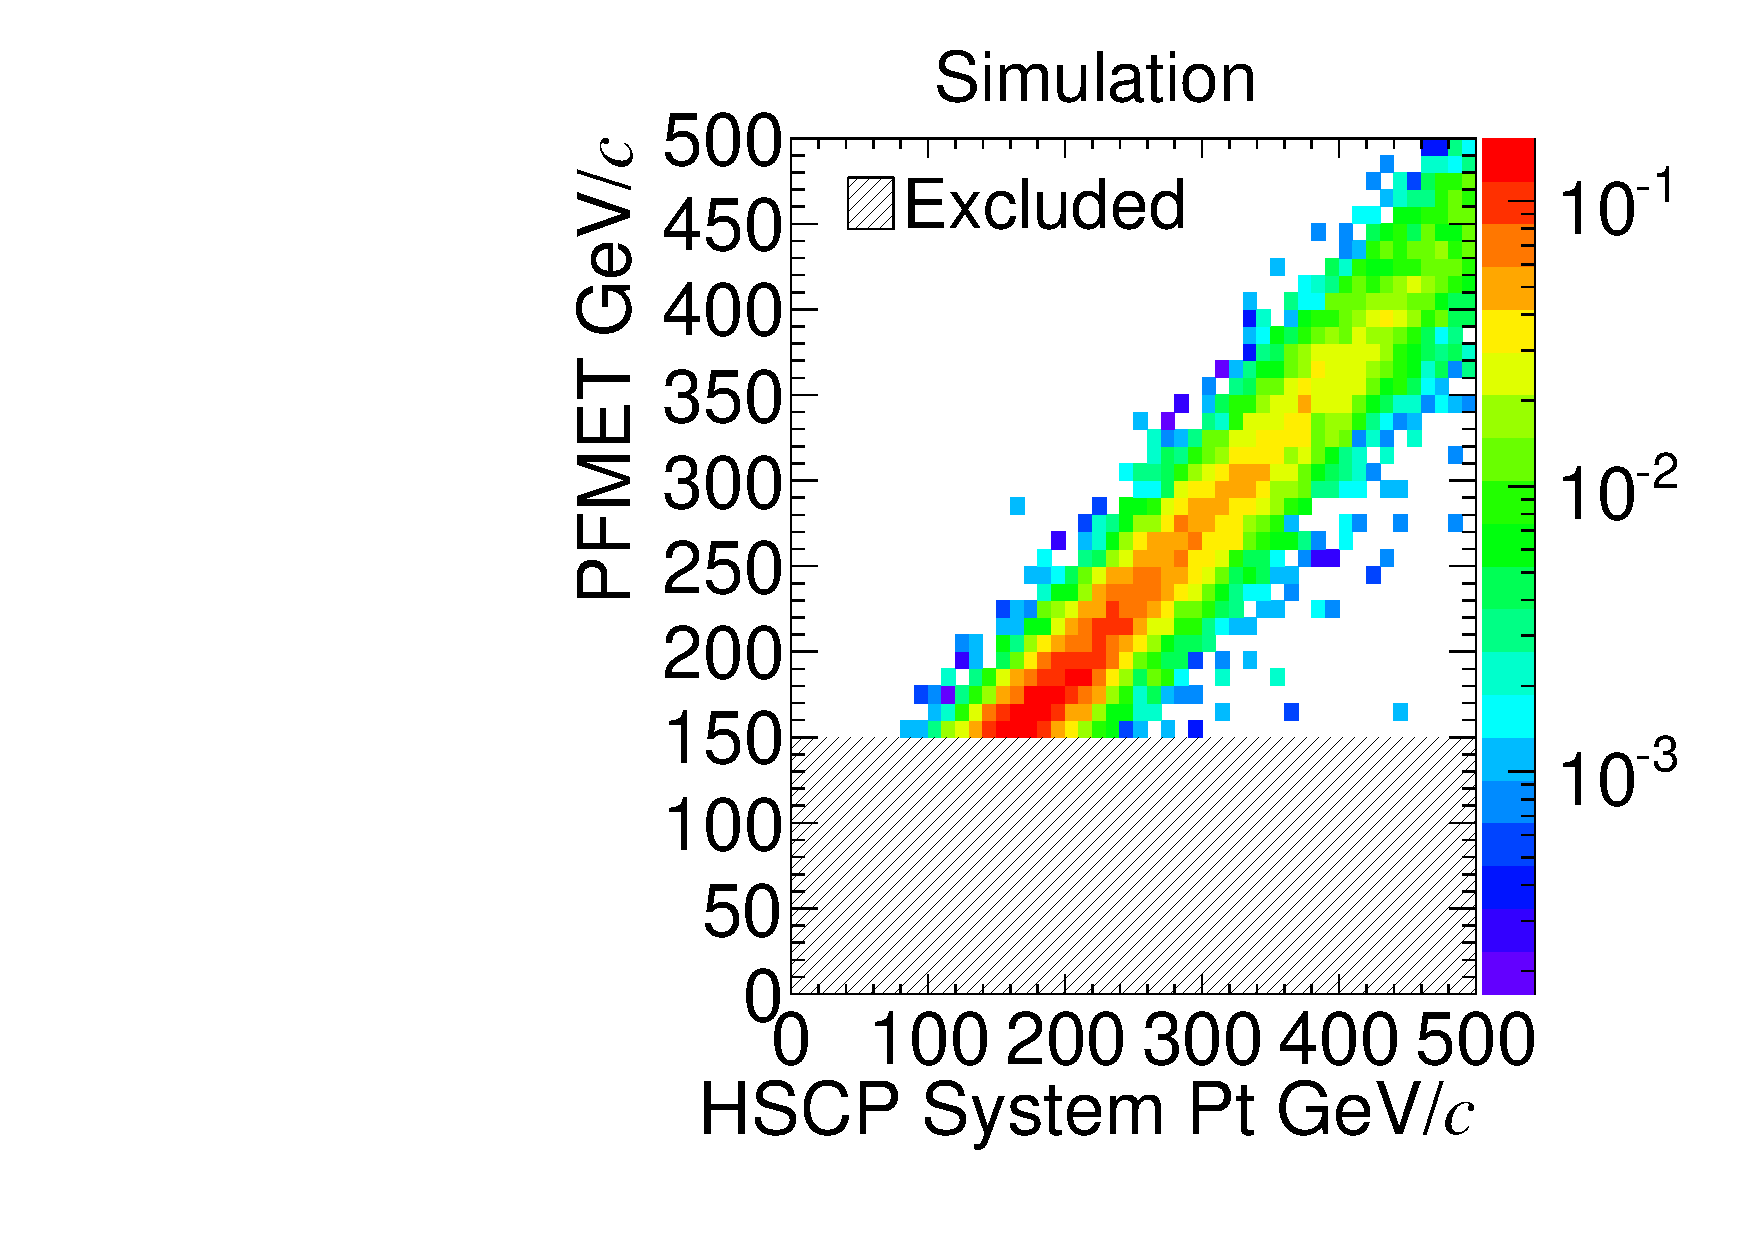
\includegraphics[clip=false, trim=0.0cm 0cm 0.0cm 0cm, width=0.49\textwidth]{figures/search/Gluino_8TeV_M1200N_f10SystPtMET} \\
      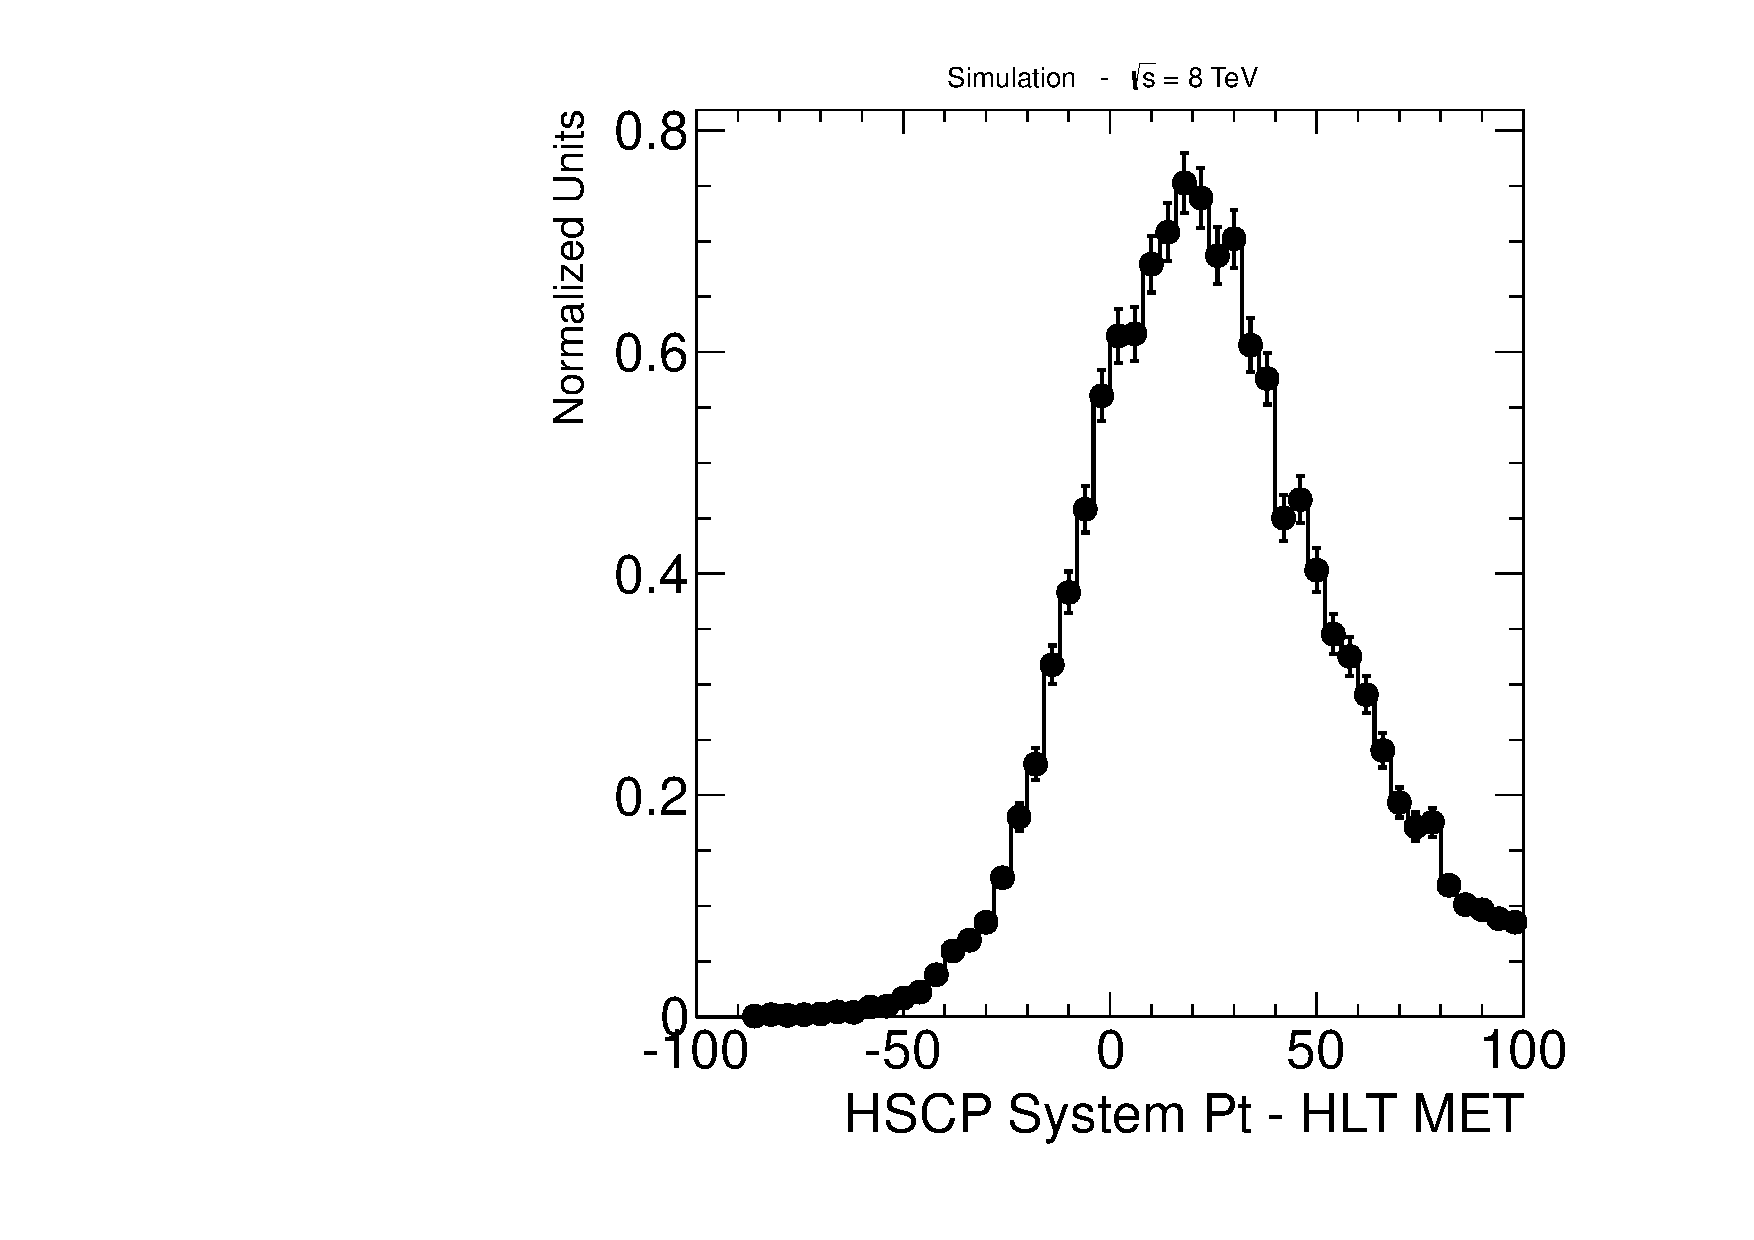
\includegraphics[clip=false, trim=0.0cm 0cm 0.0cm 0cm, width=0.49\textwidth]{figures/search/Gluino_8TeV_M1200N_f10SystPtDiffMET}
      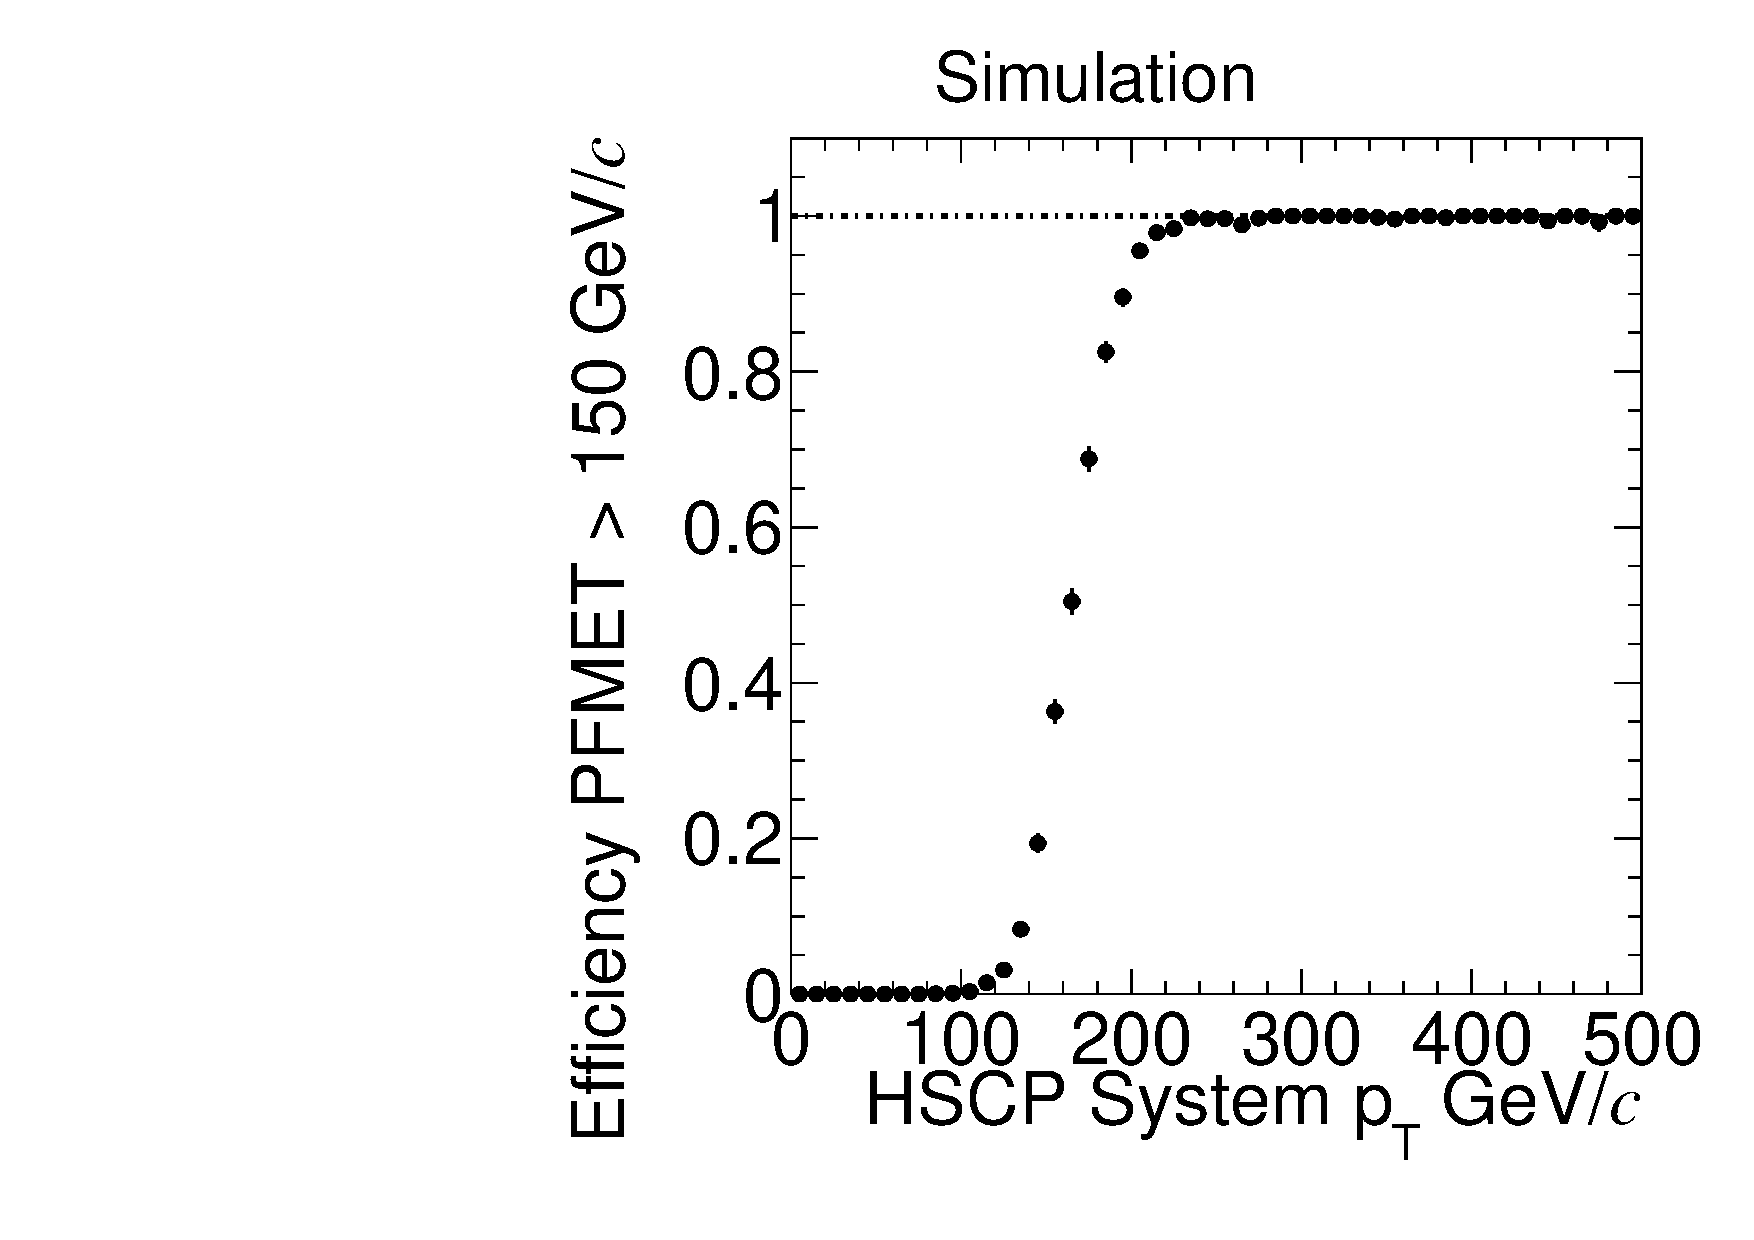
\includegraphics[clip=false, trim=0.0cm 0cm 0.0cm 0cm, width=0.49\textwidth]{figures/search/Gluino_8TeV_M1200N_f10SystPtEff}
      \caption[Comparison of di-HSCP system $\phi$ and \pt\ with PFMET for a 1200~GeV/$c^2$
gluino $f=0.1$ charge suppressed sample in events with at least 150~GeV/$c$ of PFMET]
      {Same as Fig.~\ref{fig:SystPtTrigger} but the sample used is 1200~GeV/$c^2$ $f=0.1$ charge suppressed gluino.
        }
      \label{fig:SystPtTriggerN}
  \end{center}
\end{figure}

Another trigger issue unique to slow-moving particles is the timing acceptance of the L1 trigger. If an HSCP arrives in the muon system too late, it can trigger the
readout of the wrong bunch crossing. As most of the CMS subdetectors, though not the muon system, are designed to not readout data coming from adjacent bunch crossings,
the data from the correct bunch crossing would be lost. To help deal with this, members of the CMS L1 trigger team developed a special configuration of the
RPC L1 trigger to partially recover HSCP that arrive in the muon system in the bunch crossing window following the crossing that produced them.
This configuration is discussed in Sec.~\ref{sec:computing}.

%The configuration creates a duplicate copy of all RPC hits and sends them to the muon trigger in the bunch crossing immediately preceding the arrival of the hits. 
%This allows for HSCP that
%arrive in the RPCs 0.5 -- 1.5 bunch crossings later than a collision muon would to still trigger the readout of the correct event. For particles that arrive in the RPC
%in the correct bunch crossing, a coincidence with the LHC beam crossing through CMS is required to prevent the readout of the previous event. This configuration
%was possible for 2012 running as the proton bunches were separated by 50ns despite having 25ns wide bunch crossing window windows.
%The configuration is described in more detail in Sec.~\ref{sec:computing}.

The first trigger used, L2Mu+MET, requires both a high-momentum track to be found in the muon system and large PFMET.
The algorithm starts at the L1 step where a track must be found in the muon system by the detector electronics with a momentum greater than 16~GeV/$c$ and $|\eta|$ less than 2.1 
in order to trigger the readout of the event to the computing farm.
There, the L1 track is used to seed the reconstruction of the track in the L2 step using only data readout from the muon system.
The track is required to have $p_T > 70$~GeV/$c$, $|\eta| < 2.1$, and hits in at least two muon stations.
In the L3 step, the particle flow algorithm is run and the calculated PFMET must be greater than 55 GeV/$c$.
For the first 0.7~fb$^{-1}$ of 2012 running the threshold on PFMET was at 65~GeV/$c$. The signal samples are weighted
to account for the amount of data taken at each threshold.
The lack of a requirement that the track be found in the silicon tracker allows the trigger to be sensitive to $R$-hadrons produced neutral and only later becoming charged.
The main objective of the PFMET requirement is to reduce the rate of events collected by the trigger.
The momentum measurement by the muon system suffers from long tails and the rate would be too large even with a very high momentum threshold.
With the PFMET requirement, the cross-section of the trigger is approximately 0.3~$\mu$b.
Events collected with this trigger are only used in the \muononly\ analysis.

The second trigger used, Mu40, requires a high momentum track matched in both the silicon tracker and muon system be found.
During the L1 and L2 steps, the algorithm follows the same procedure as the L2Mu+MET trigger, with the only difference being the $p_T$ threshold on the L2 track
is reduced to 16~GeV/$c$ and only one muon station is required to have hits.
During the L3 step, the L2 track is used to seed the reconstruction of tracks that span from the silicon tracker to the muon system.
A track must be found with momentum greater than 40~GeV/$c$ and $|\eta|$ less than 2.1. The very good resolution of the silicon tracker allows for an acceptable trigger rate
without any further requirements. 
The cross-section of the trigger is approximately 3.5~$\mu$b.
Events collected with this trigger are used in all analyses.

The third trigger used, PFMET150, requires at least 150~GeV/$c$ of PFMET be found at the L3 step. The L1 and L2 steps of the trigger calculate the MET in the event using
only the energy deposits in the calorimeter, a faster method than particle flow, and apply looser requirements on the MET of 40 and 80~GeV/$c$, respectively.
The cross-section of the trigger is approximately 0.6~$\mu$b.
Events collected with this trigger are used in all analyses.

The decision to use the pure PFMET trigger even when a muon signature is required offline is prompted by the late arrival of the HSCPs in the muon system.
Even with the RPC configuration described above, very slow moving HSCP can trigger the readout of the wrong event but still be reconstructed offline
if the event has been triggered by the pure PFMET trigger. This can be seen in Figure~\ref{fig:TriggerEffVsBetaGl} which shows the trigger efficiency versus $\beta$
with and without the pure PFMET trigger.
It can be seen that using the pure PFMET trigger allows the search to probe lower $\beta$ particles. 

%Additional triggers were developed to collect - Maybe add dE/dx triggers?

%As color charged $R$-hadron can be neutral
%while traversing CMS or arrive so late to the muon system that they are not able to be reconstructed offline an effective detector acceptance is defined 
%that at least one HSCP be reconstructed offline. Thus Figure~\ref{fig:TriggerEffVsBetaGl} shows the efficiency requiring an HSCP be reconstructed as a track
%as in the \muononly\ analysis, and as a global track, as in the the \tktof\ analysis.

\begin{figure}
\centering
%  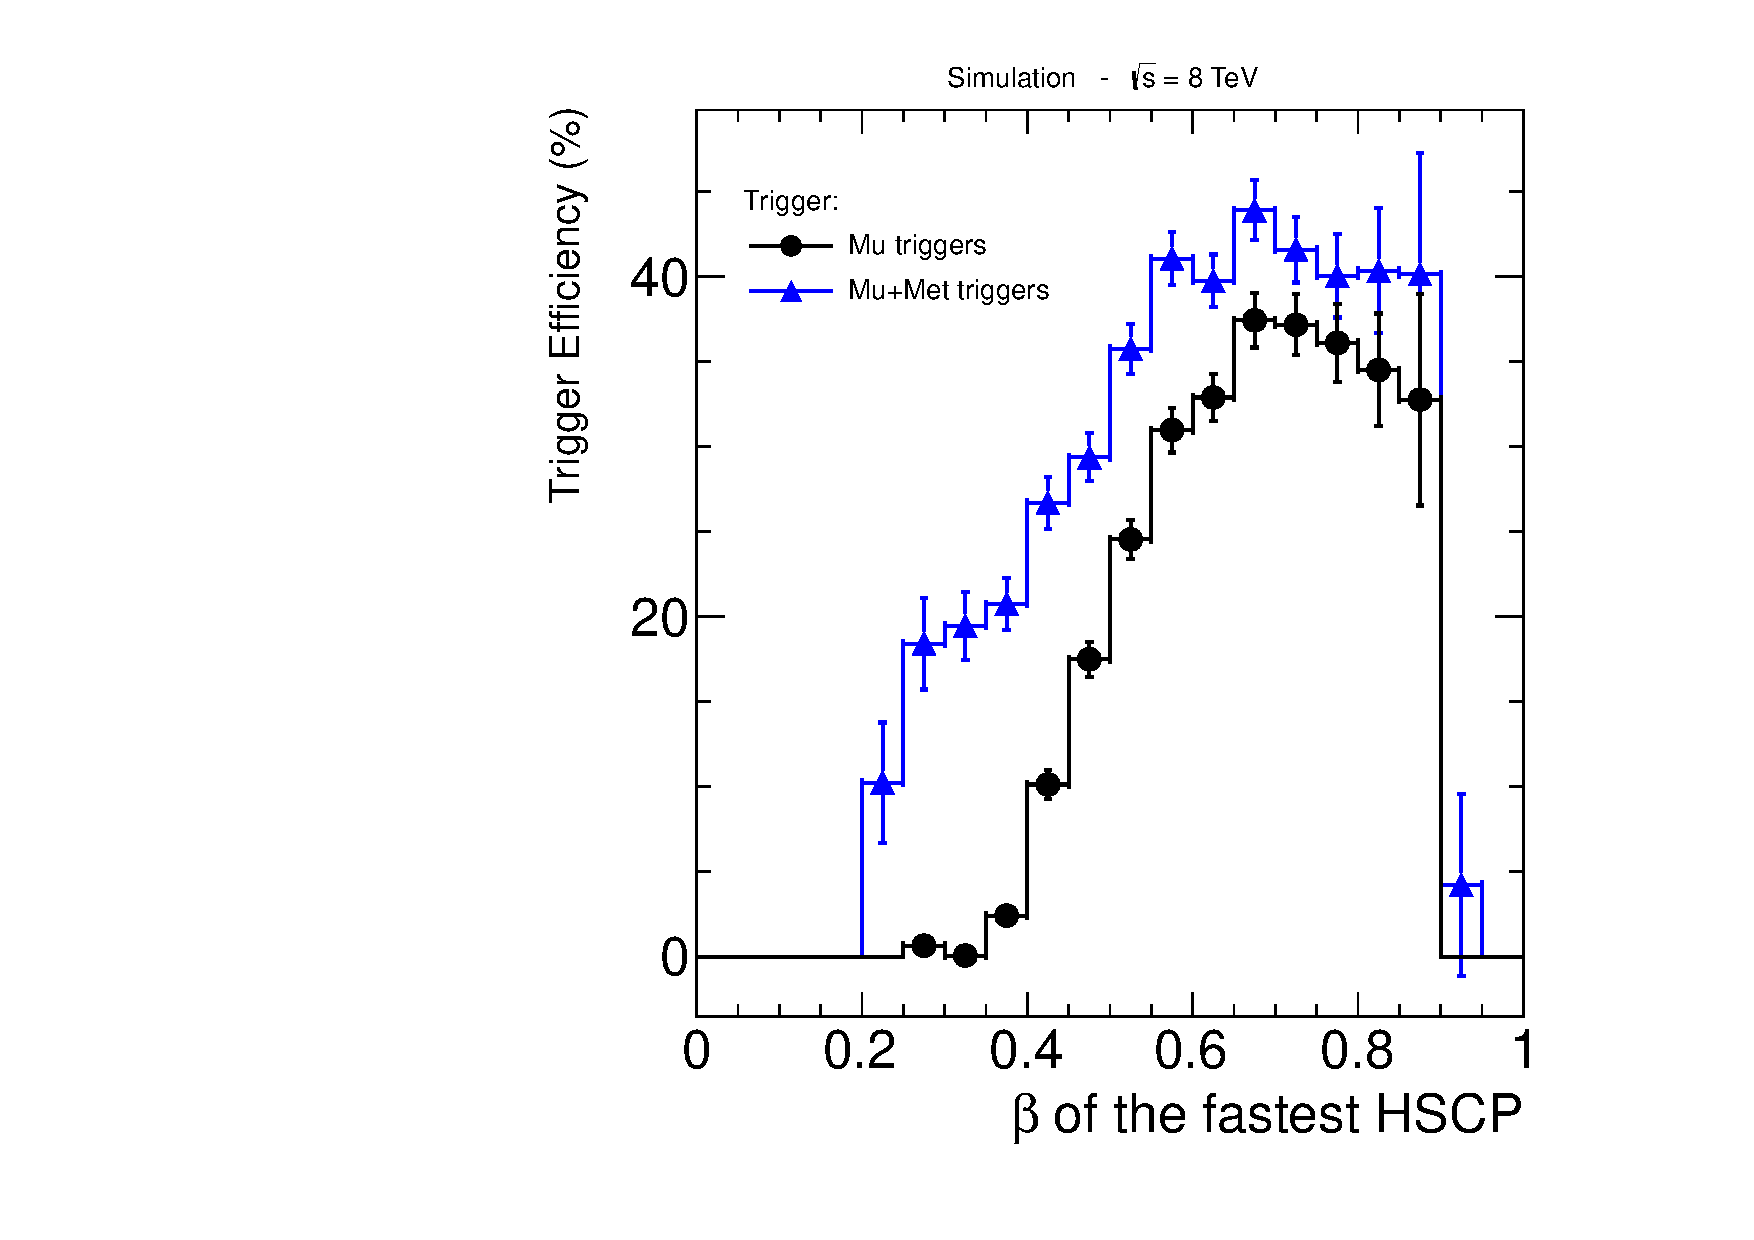
\includegraphics[clip=true, trim=0.0cm 0cm 3.0cm 0cm, width=0.49\textwidth]{figures/search/Gluino_8TeV_M1200_f100MatchedSA}
  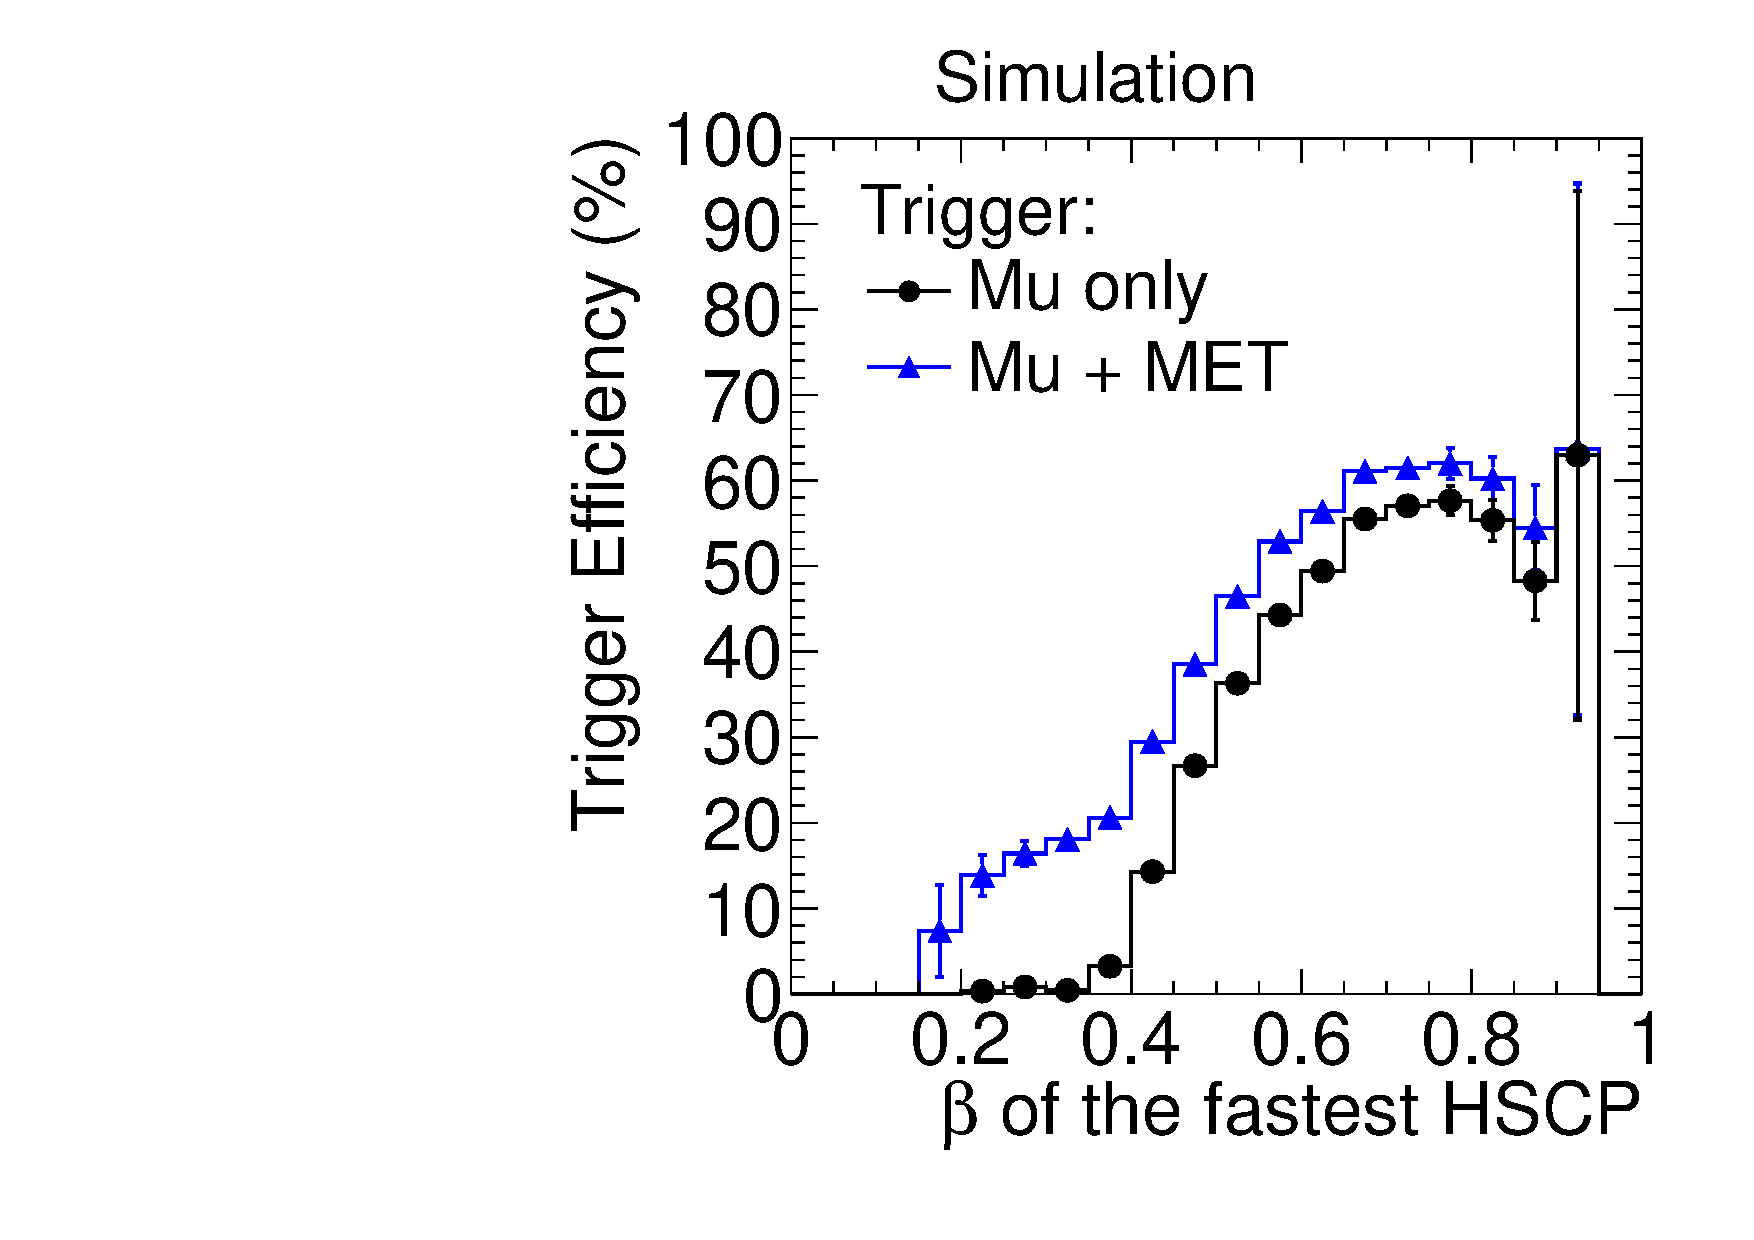
\includegraphics[clip=false, trim=0.0cm 0cm 0.0cm 0cm, width=0.49\textwidth]{figures/search/Gluino_8TeV_M1200_f10MatchedSA}
  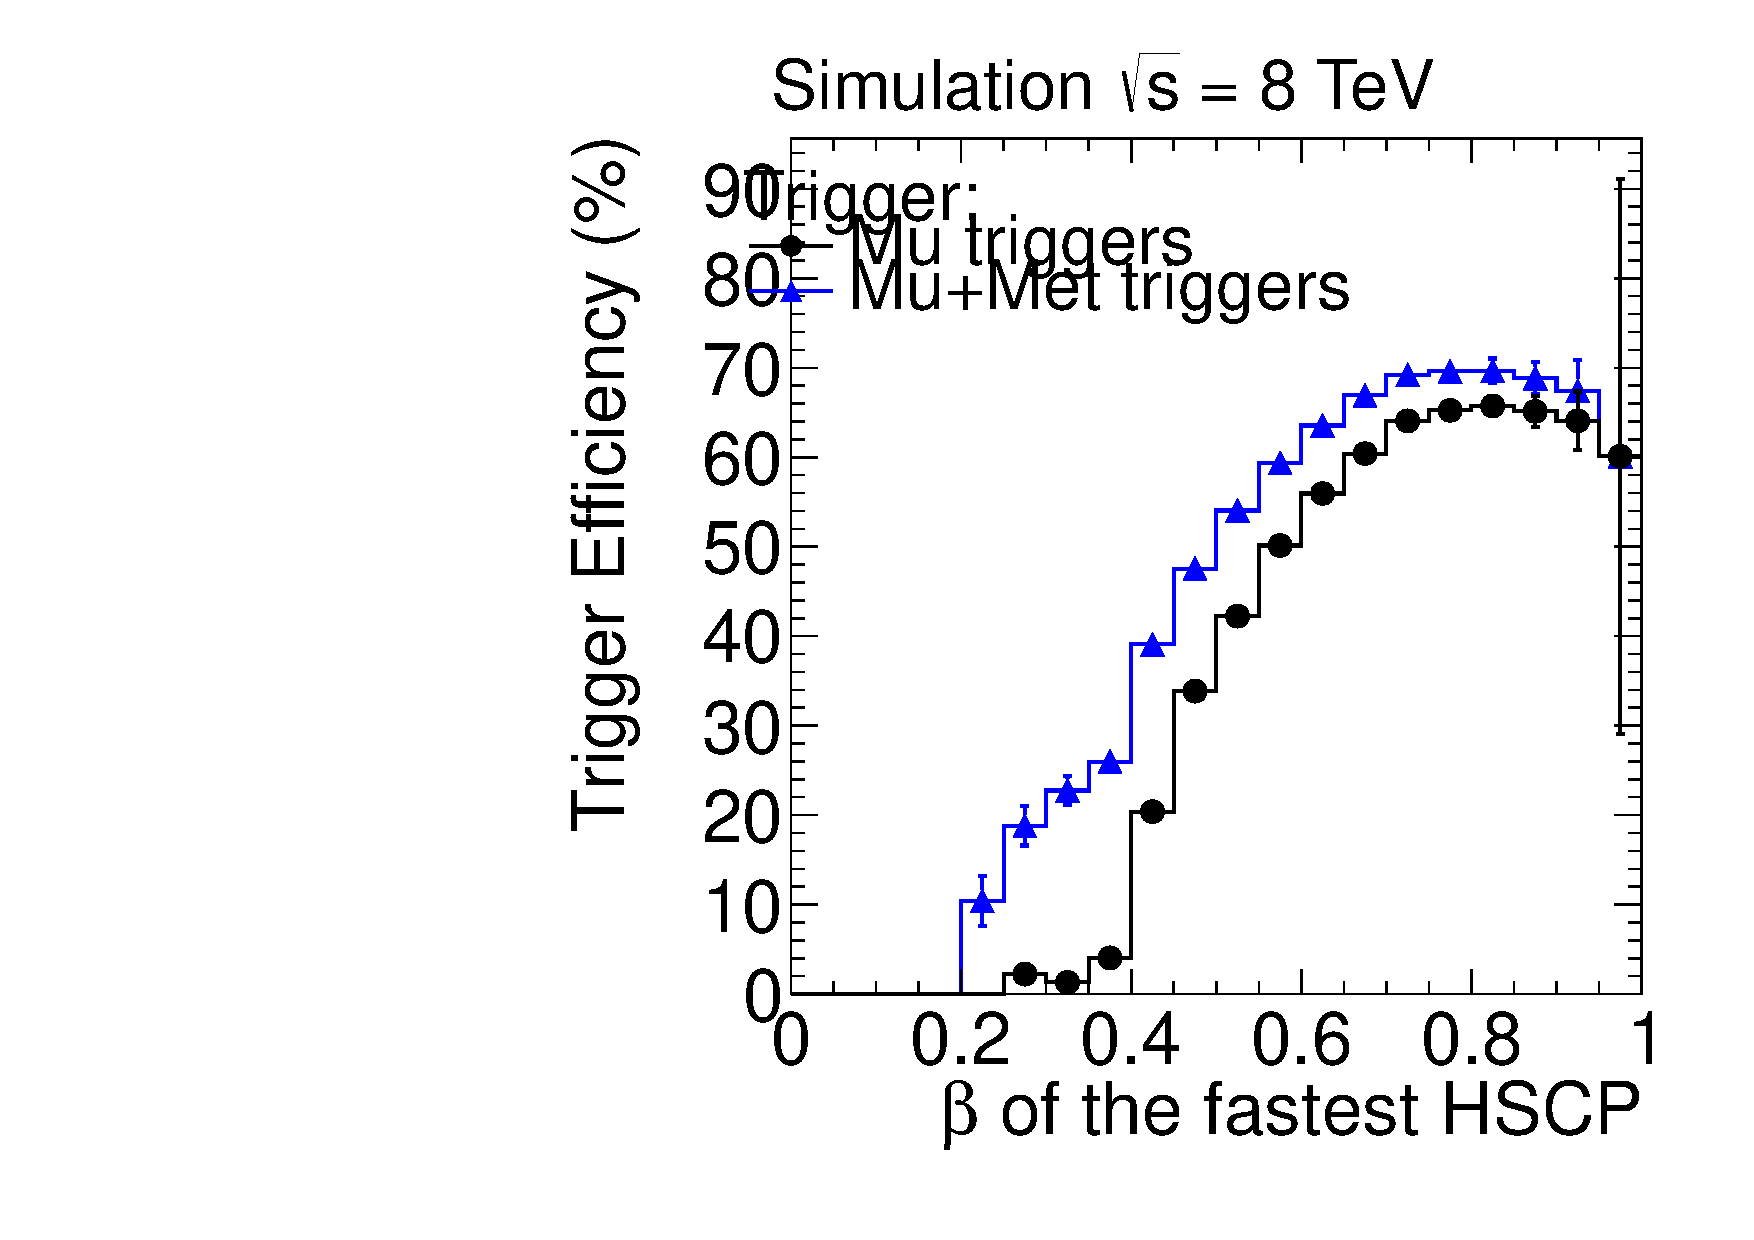
\includegraphics[clip=false, trim=0.0cm 0cm 0.0cm 0cm, width=0.49\textwidth]{figures/search/Stop_8TeV_M800MatchedSA}
%  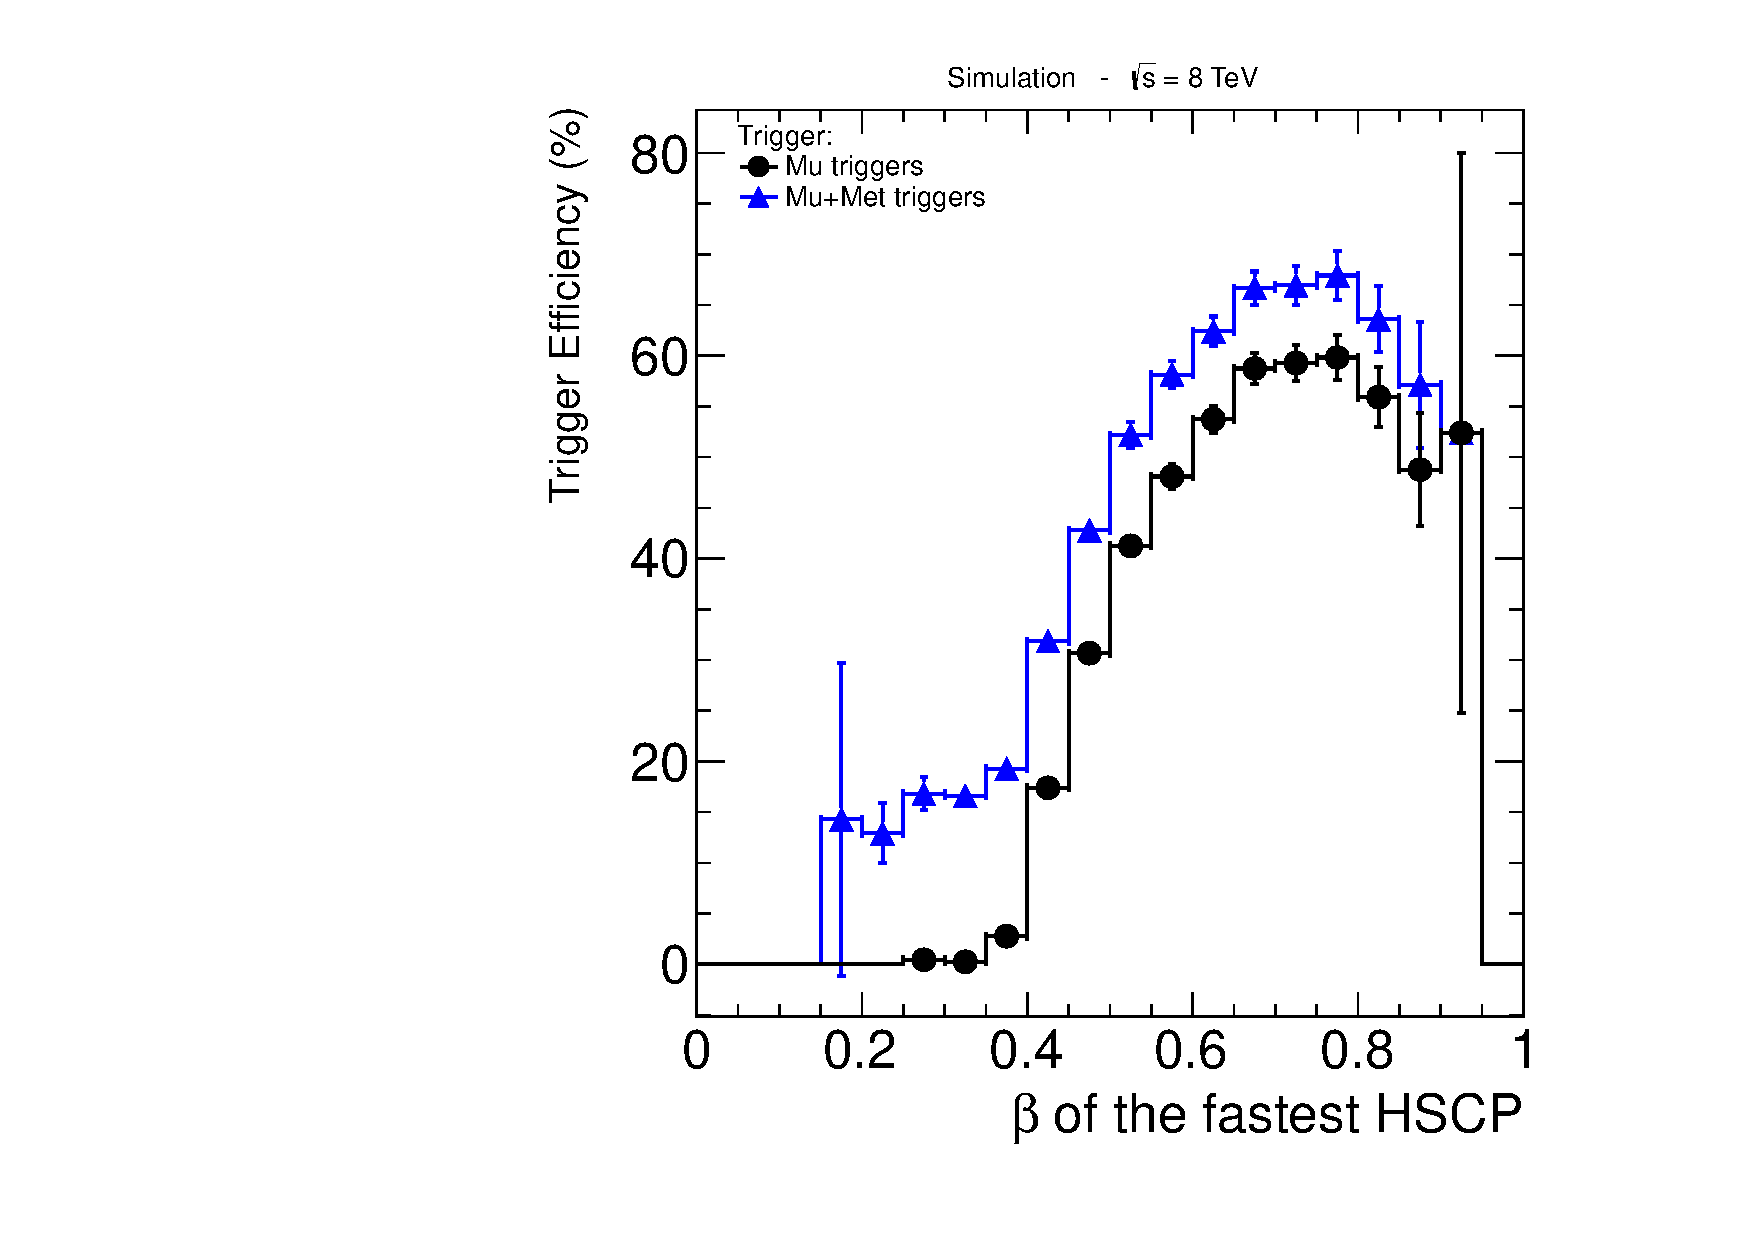
\includegraphics[clip=true, trim=0.0cm 0cm 3.0cm 0cm, width=0.32\textwidth]{figures/search/Gluino_8TeV_M1200_f10MatchedGl}
%  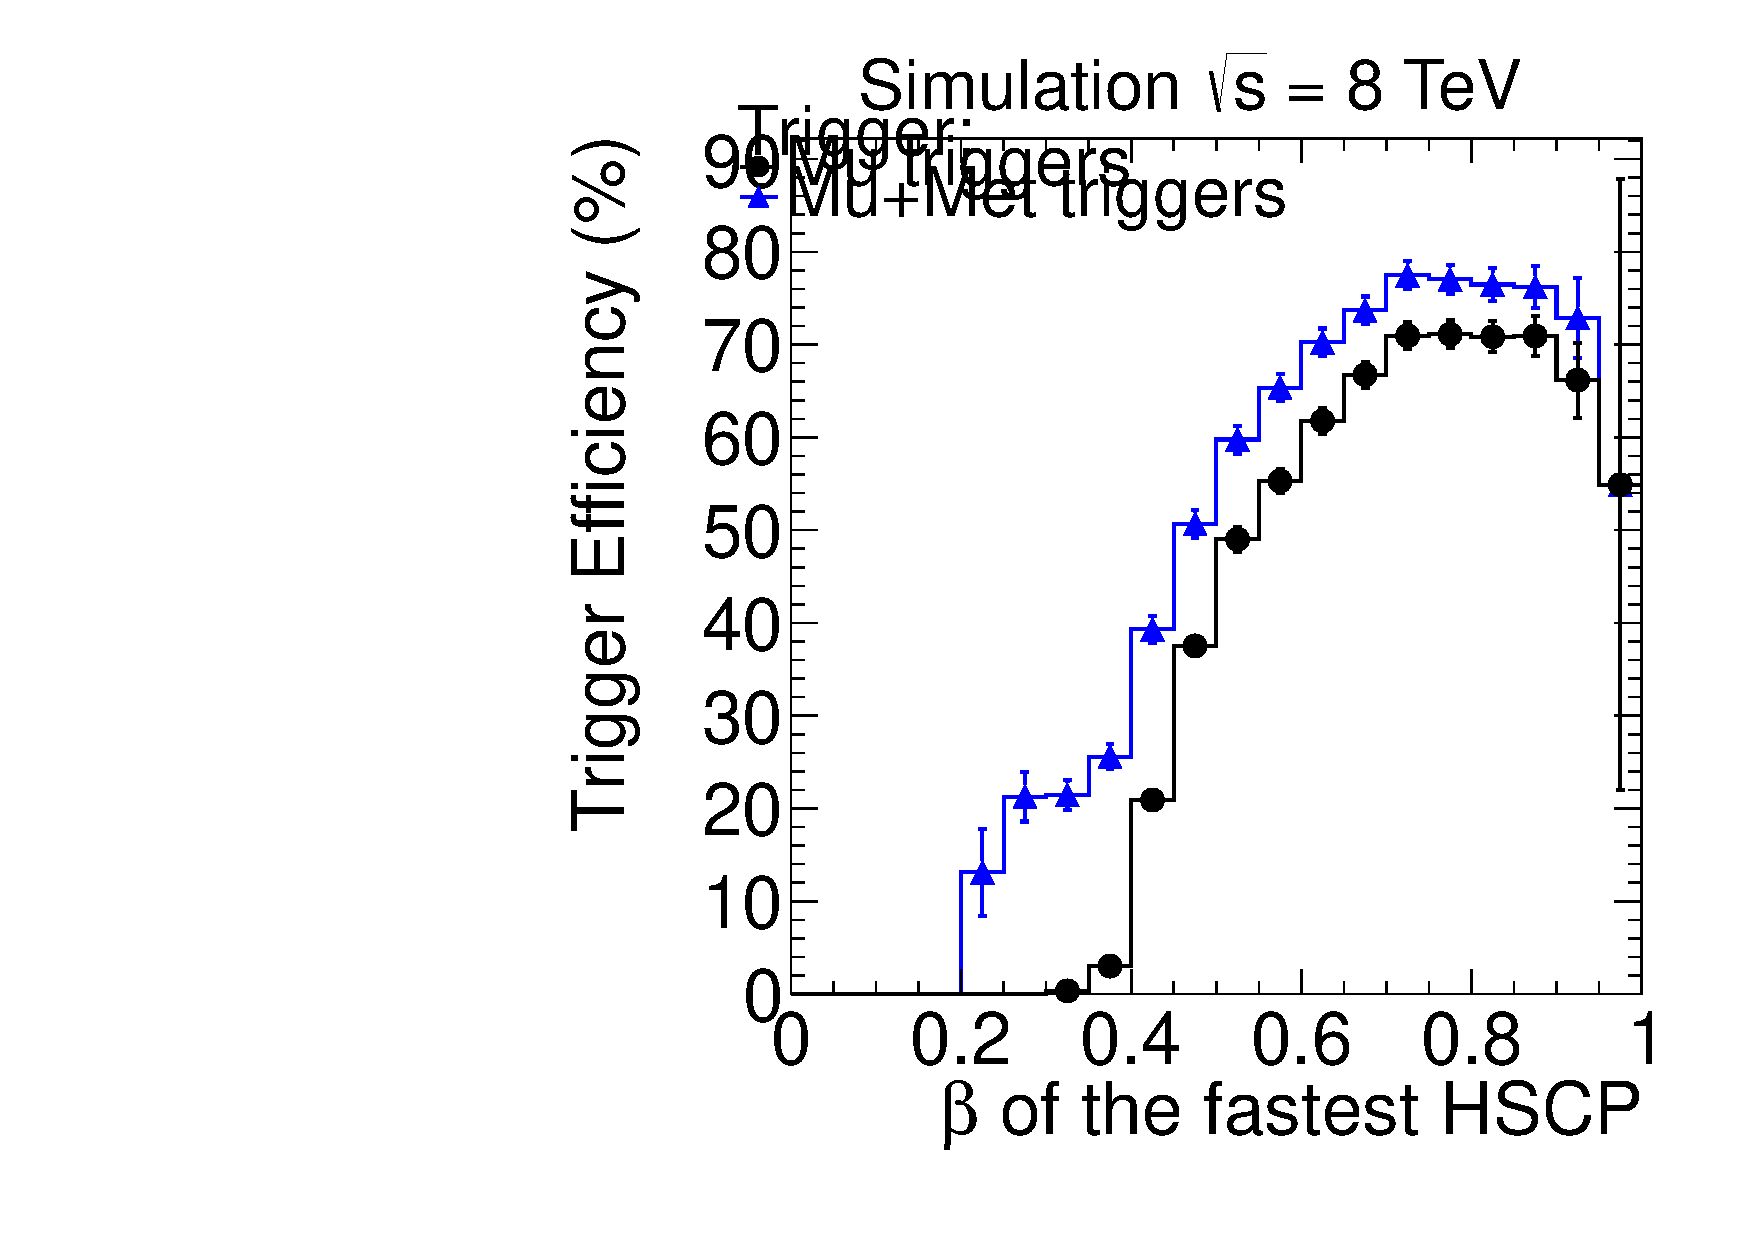
\includegraphics[clip=true, trim=0.0cm 0cm 3.0cm 0cm, width=0.32\textwidth]{figures/search/Stop_8TeV_M800MatchedGl}
%  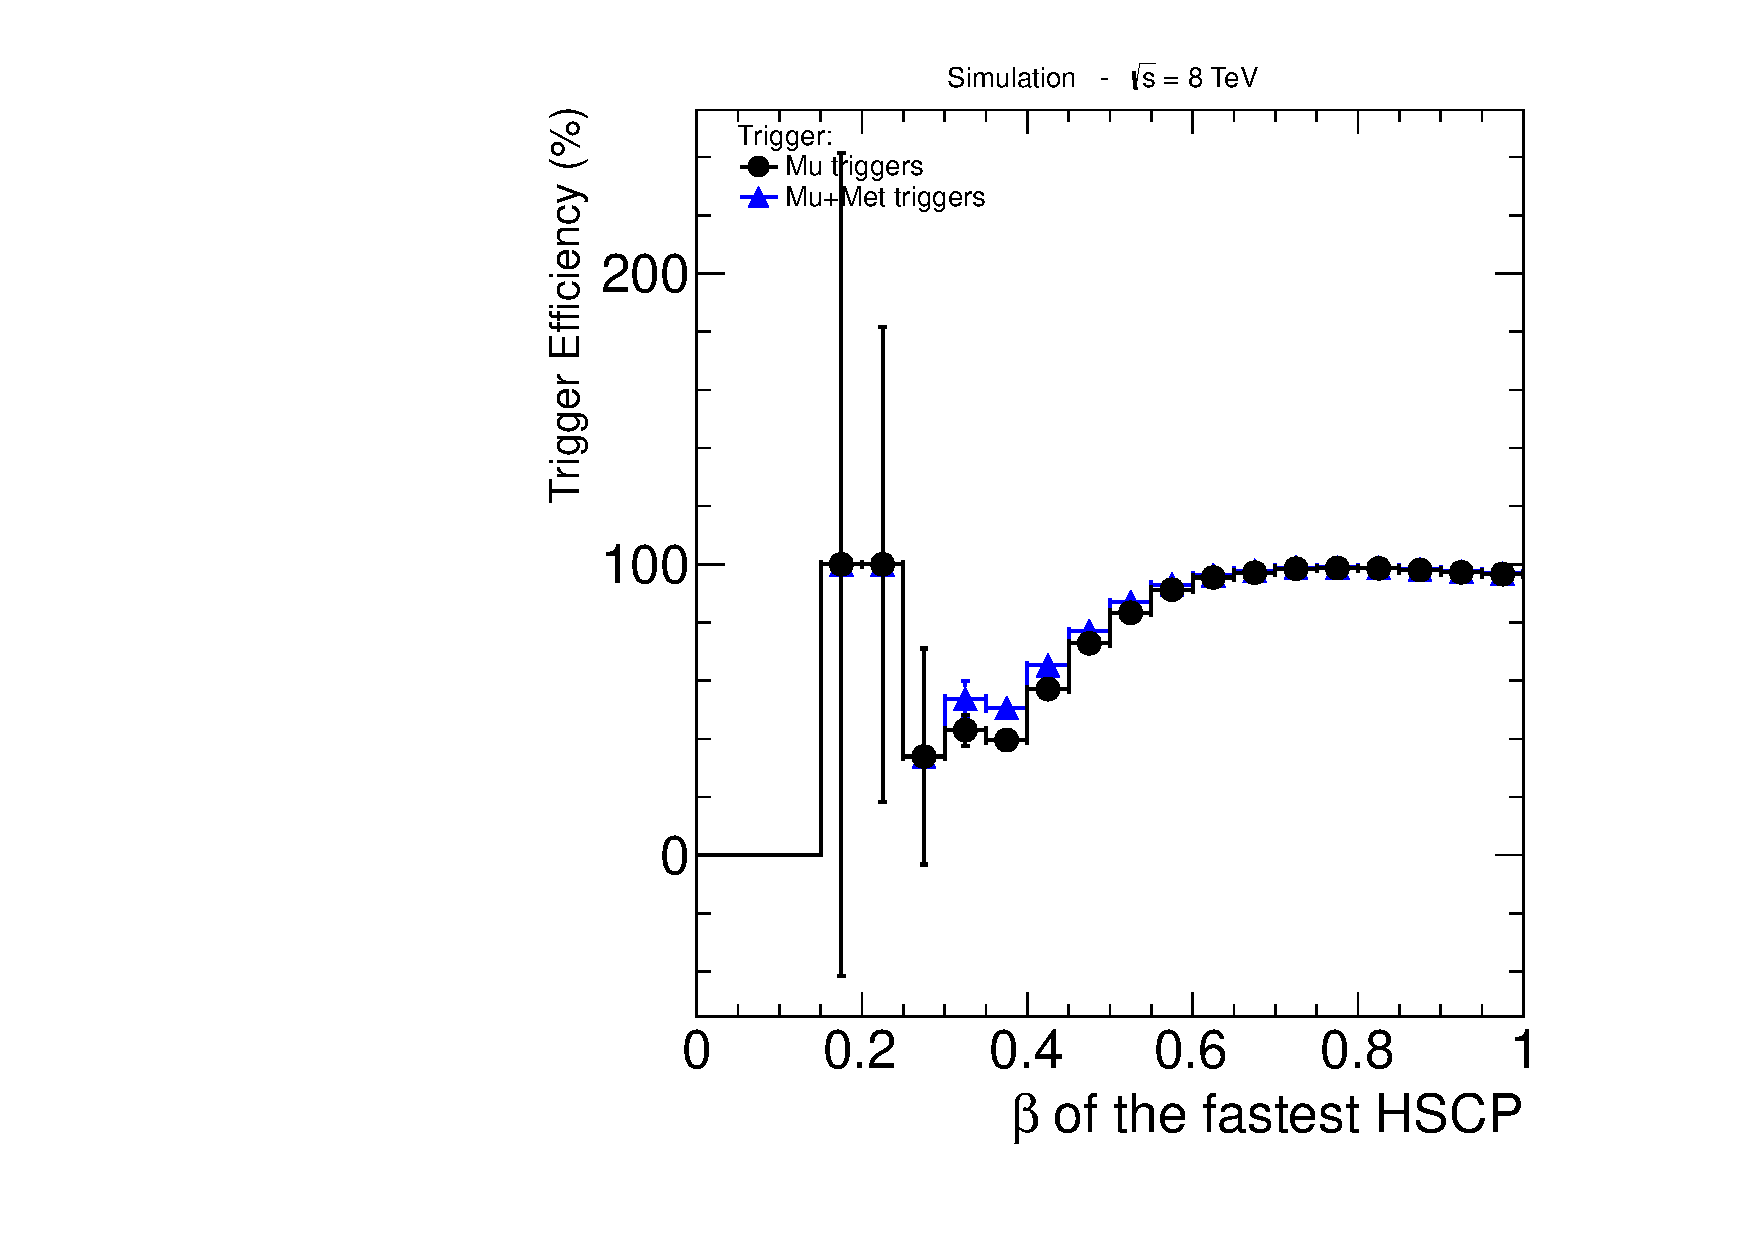
\includegraphics[clip=true, trim=0.0cm 0cm 3.0cm 0cm, width=0.32\textwidth]{figures/search/GMStau_8TeV_M494MatchedGl}
      \caption[Trigger efficiency as a function of the $\beta$ of the fastest HSCP reconstructed offline in the muon system with only the muon triggers
and additionally including the PFMET trigger.]
{Trigger efficiency as a function of the $\beta$ of the fastest HSCP reconstructed offline in the muon system with only the muon triggers
and additionally including the pure PFMET trigger.
The samples are 1200~GeV/$c^2$ Gluino $f=0.1$ (left) and 800~GeV/$c^2$ stop (right).}
    \label{fig:TriggerEffVsBetaGl}
\end{figure}

When evaluating trigger efficiencies, it is important to only consider events that have a possibility of being selected offline.
For the case of strongly charged HSCP this is made more difficult as some events may not have any $R-hadrons$ electrically charged while they pass through the detector.
To deal with this, the trigger efficiencies are reported with respect to events where at least one HSCP is found offline.
The efficiency for each trigger, as well as the combined efficiency, is listed for various signal samples in Tables~\ref{tab:triggEffSA} and ~\ref{tab:triggEffGl} in events
with at least one HSCP reconstructed in the muon system and the muon system plus the silicon tracker, respectively. The simulation has been found to 
provide a good modeling of  muon reconstruction~\cite{2012JInst...7P0002T} and MET determination~\cite{CMS-PAS-JME-12-002} by CMS.
Further discussion of possible residual differences between simulation and data can be found in Sec.~\ref{sec:SystUnc}.

\begin{table}
 \begin{center}
  \caption[Trigger efficiency for various models considered with respect to events with a reconstructed HSCP in the muon system]
{Efficiency in percentage for various models for the L2Mu+MET, Mu40, PFMET150 triggers and a combination of the three.
The efficiencies are with respect to events with at least one HSCP reconstructed in the muon system.}
     \label{tab:triggEffSA}
  \begin{tabular}{|l|c|c|c|c|c|} \hline
      Model     & Mass (GeV/$c^2$) &L2Mu+MET & Mu40       & PFMET150   & Total   \\ \hline
 Gluino $f=0.1$ &  400       & 34.3    & 35.6       & 19.4       & 58.6    \\
 Gluino $f=0.1$ &  800       & 31.2    & 31.6       & 22.6       & 54.9    \\
 Gluino $f=0.1$ & 1200       & 24.6    & 26.6       & 20.5       & 47.5    \\
 Gluino $f=1.0$ &  400       & 36.6    & 5.6        & 23.2       & 46.1    \\
 Gluino $f=1.0$ &  800       & 31.9    & 5.0        & 24.5       & 43.4    \\
 Gluino $f=1.0$ & 1200       & 23.6    & 3.7        & 20.6       & 35.5    \\
           Stop &  200       & 27.3    & 42.8       & 11.2       & 58.8    \\
           Stop &  500       & 31.1    & 42.1       & 19.8       & 61.2    \\
           Stop &  800       & 30.3    & 41.6       & 21.6       & 60.7    \\ \hline
  \end{tabular}
 \end{center}
\end{table}

\begin{table}
 \begin{center}
      \caption[Trigger efficiency for various models considered with respect to events with a reconstructed HSCP in both the muon system and inner tracker]
	      {Efficiency in percentage for various models for the Mu40, PFMET150, triggers and a combination of the two.
The efficiencies are with respect to events with at least one HSCP reconstructed in both the muon system and inner tracker.}
     \label{tab:triggEffGl}
  \begin{tabular}{|l|c|c|c|c|} \hline
      Model     & Mass (GeV/$c^2$) & Mu40       & PFMET150   & Total                 \\ \hline
 Gluino $f=0.1$ &  400       & 51.87      & 16.06      & 59.09    \\
 Gluino $f=0.1$ &  800       & 46.50      & 20.50      & 56.42    \\
 Gluino $f=0.1$ & 1200       & 38.96      & 19.56      & 49.95    \\
           Stop &  200       & 58.43      &  7.69      & 61.54    \\
           Stop &  500       & 56.91      & 17.40      & 64.44    \\
           Stop &  800       & 56.15      & 20.49      & 65.59    \\
        CD Stau &  100       & 97.86      & 14.74      & 98.06    \\
        CD Stau &  308       & 97.03      & 17.53      & 97.47    \\
        CD Stau &  494       & 95.56      & 17.76      & 96.35    \\
        DP Stau &  100       & 95.06      &  0.17      & 95.09    \\
        DP Stau &  200       & 95.78      &  0.37      & 95.82    \\
        DP Stau &  494       & 95.23      &  1.16      & 95.36    \\ \hline
  \end{tabular}
 \end{center}
\end{table}

Muons from cosmic rays are an important background for the \muononly\ analysis. To study and predict them, a trigger that selects events when no beams are passing through
CMS is used. The trigger requires the presence of a muon system track with $p_T > 20$~GeV/$c$, no proton bunches passing through CMS within 50ns,
and for the event not to be flagged as beam halo~\cite{wangler2000beam}.
The muon system track reconstruction used for the cosmic ray muon trigger is slightly different than for the collision trigger.
However both reconstructions are required offline as discussed in section~\ref{sec:preselection} so no bias is introduced.

Throughout the rest of this chapter, the data sample is defined to be events collected with the L2Mu+MET, Mu40, or PFMET150 triggers if in reference to the \muononly\ analysis.
For the other analyses it is defined to be events collected with either the Mu40 or PFMET150 triggers. The cosmic-ray control sample used in the \muononly\ analysis
is defined to be events collected with cosmic-ray trigger discussed above. In all following discussions or figures, simulated samples must have passed one 
or more of the triggers associated with the relevant analysis.